
\section{Activity Diagrams}

The following activity diagrams illustrate the detailed workflows for key system processes, showing the sequence of actions, decision points, and parallel activities across the Verdant Search platform.

\begin{figure}[H]
    \centering
    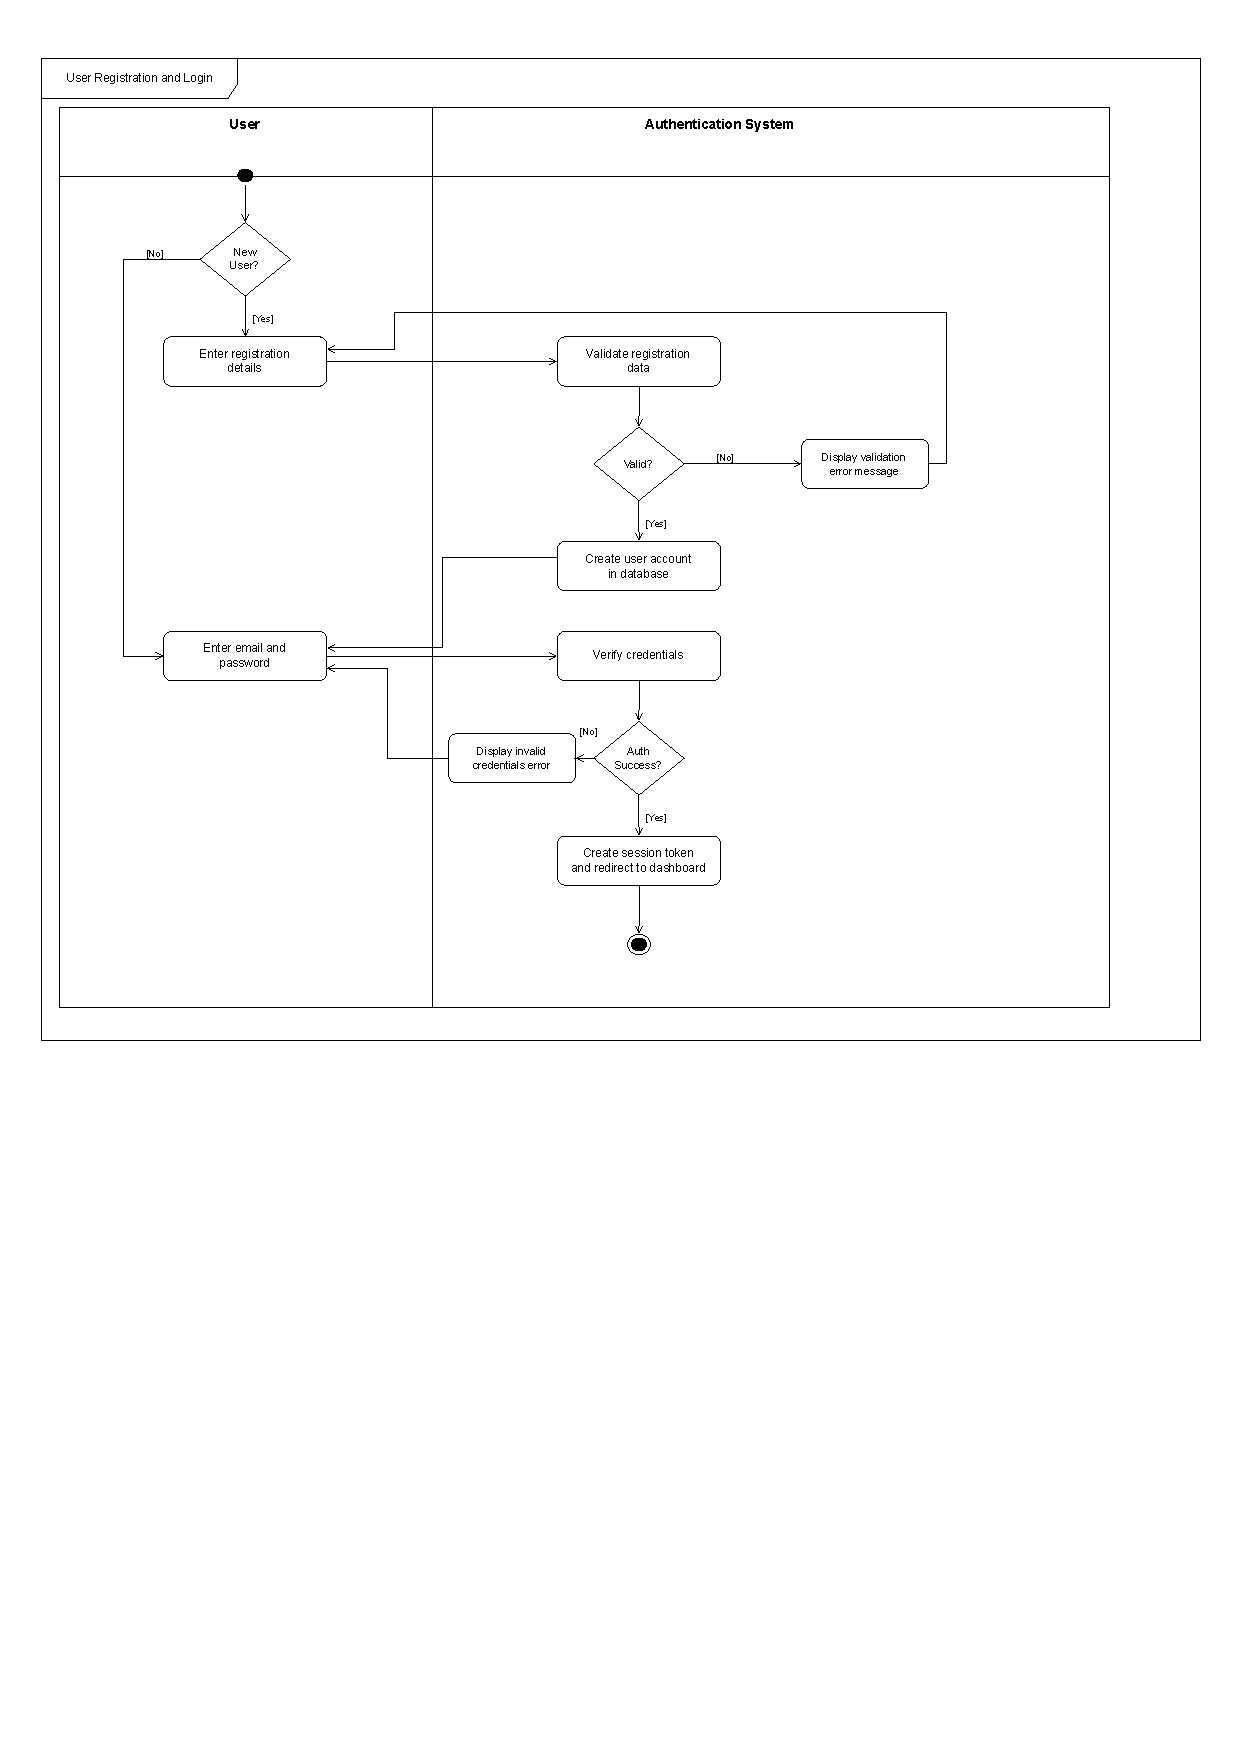
\includegraphics[width=0.55\linewidth]{activity1_fixed.drawio (3).pdf}
    \caption{Activity Diagram: User Registration and Authentication Flow}
    \label{fig:activity1}
\end{figure}

Figure \ref{fig:activity1} depicts the complete user registration and authentication workflow. The process begins when a new user accesses the registration page and submits credentials. The system validates the email format and password strength according to security requirements (minimum 8 characters with mixed case, numbers, and special characters). Upon successful validation, the system creates a hashed password using bcrypt with a cost factor of 12, stores the user account in PostgreSQL, and sends a verification email. For existing users, the authentication flow verifies credentials, generates a JWT token with 24-hour expiration, and establishes a secure session.

\begin{figure}[H]
    \centering
    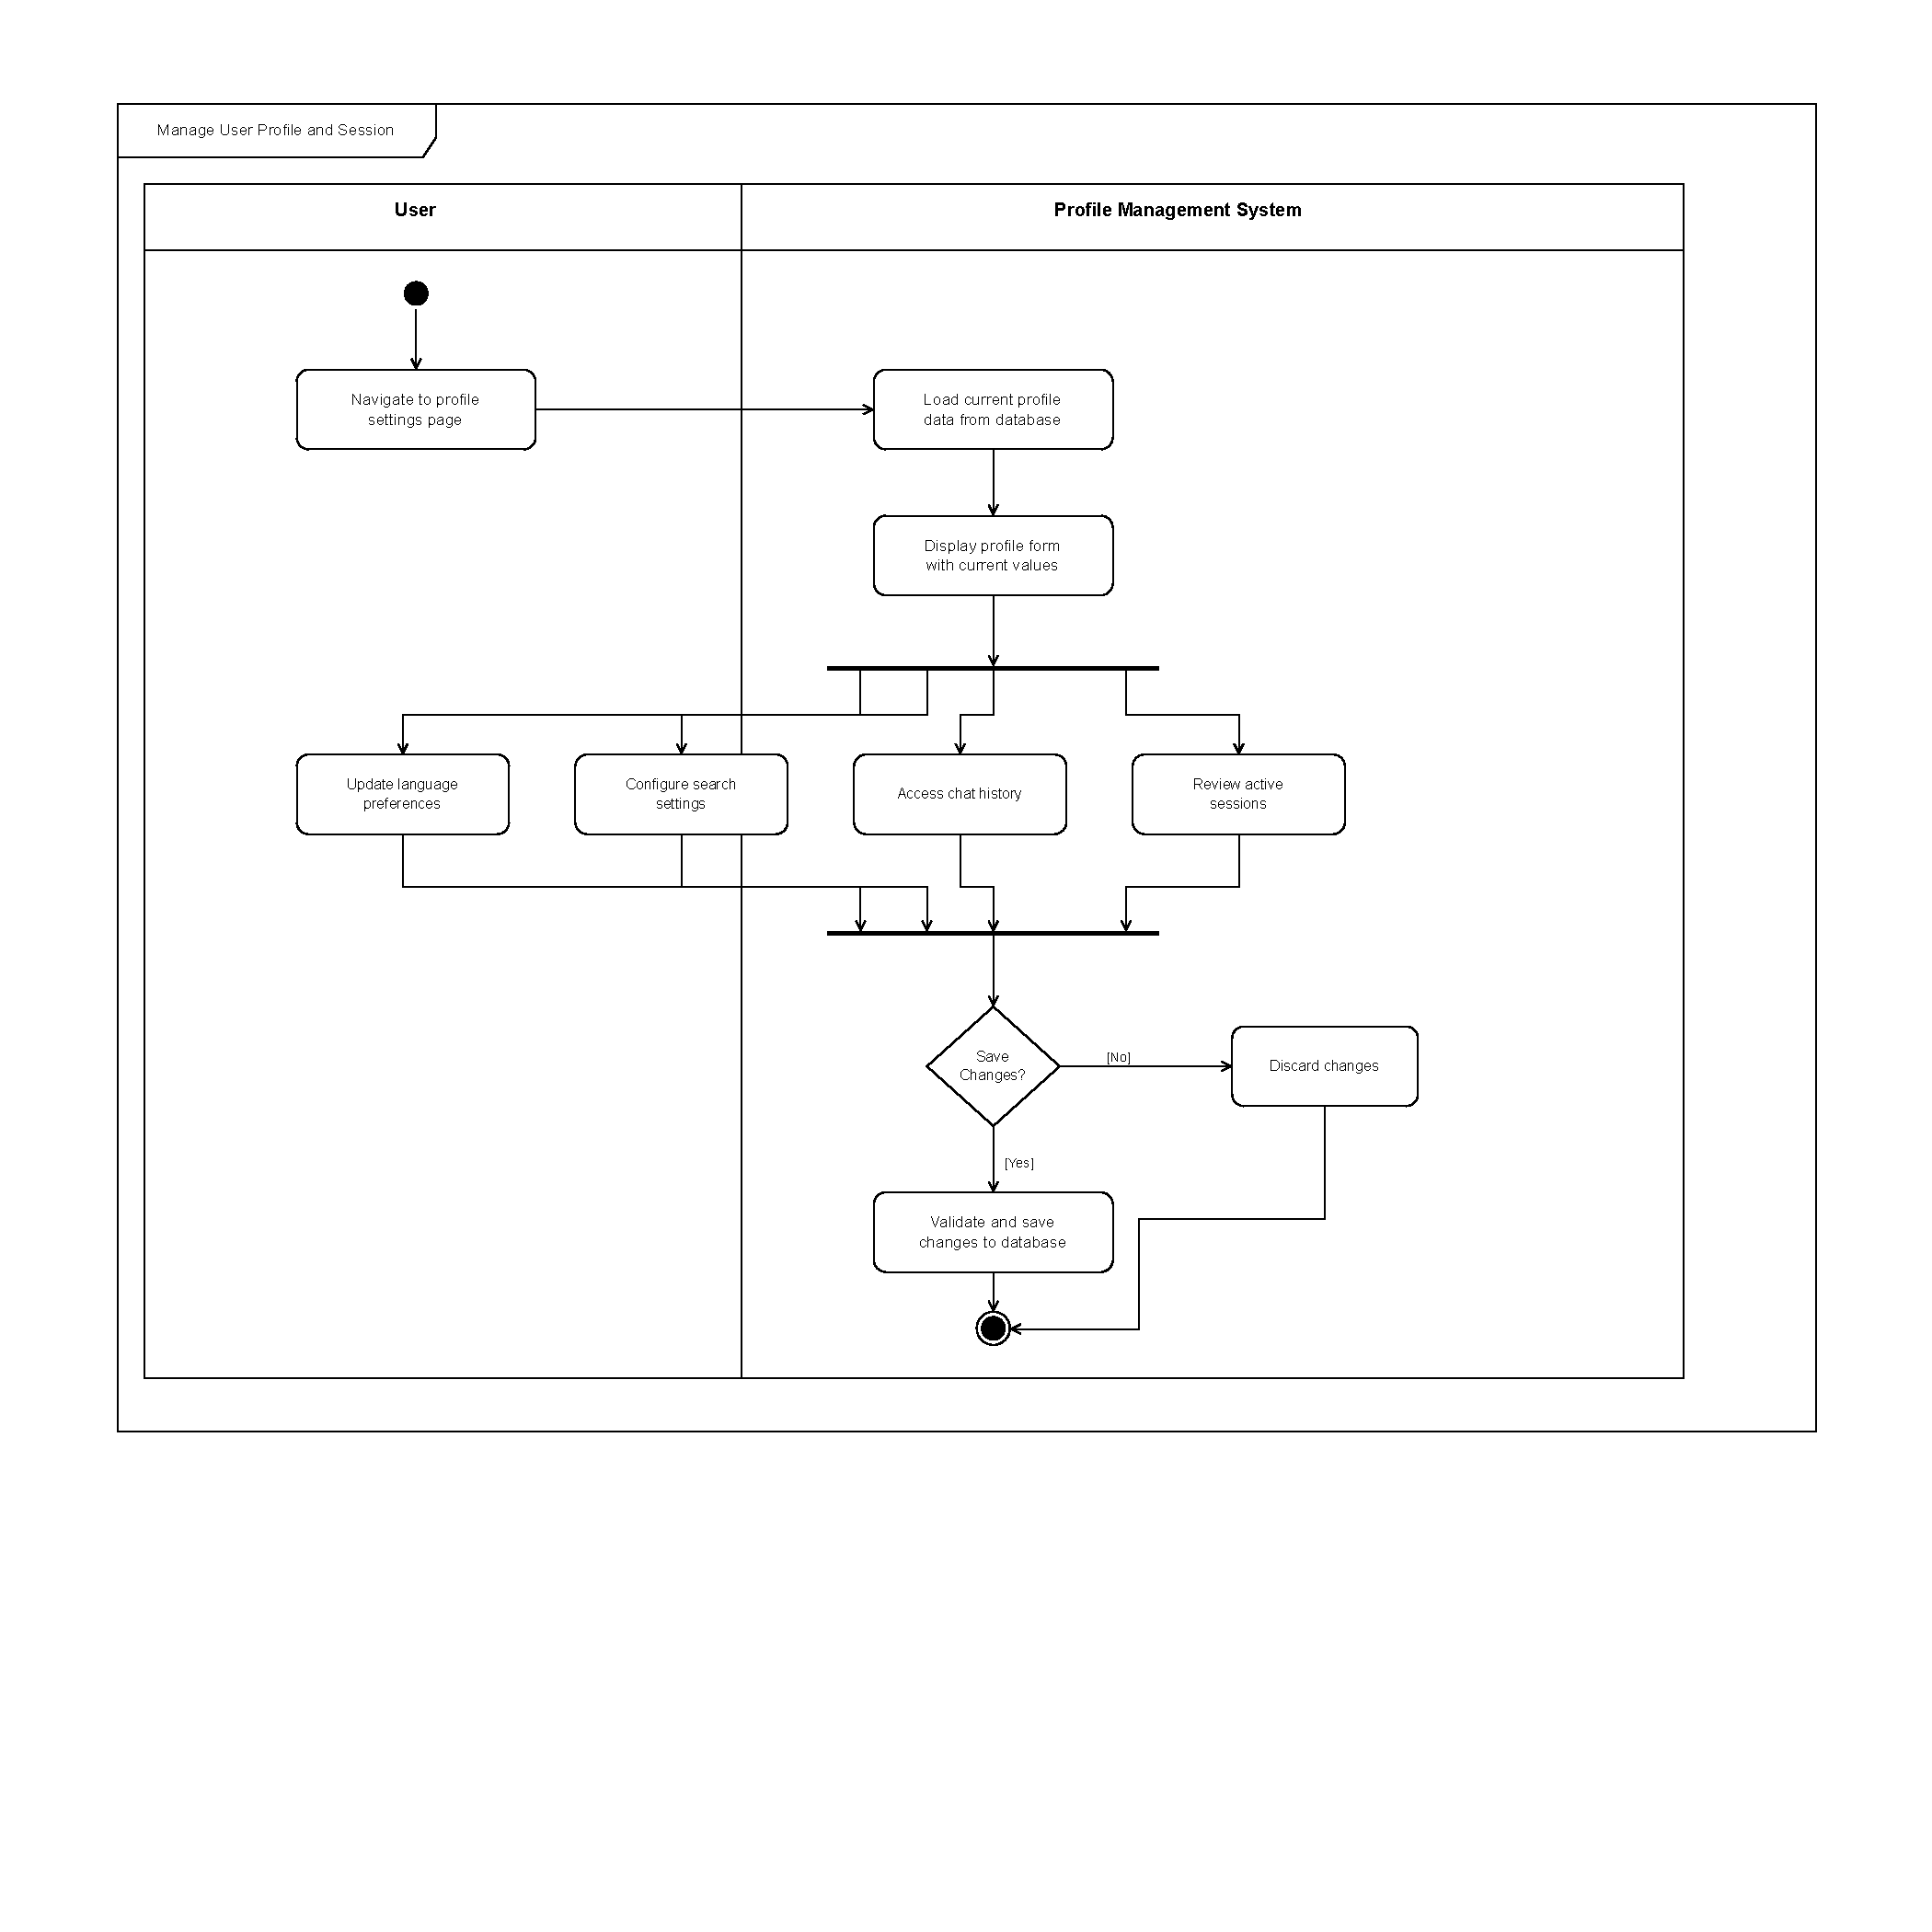
\includegraphics[width=0.55\linewidth]{activity2.drawio.pdf}
    \caption{Activity Diagram: Hybrid Search Execution Flow}
    \label{fig:activity2}
\end{figure}

Figure \ref{fig:activity2} illustrates the hybrid search execution workflow that combines BM25 keyword retrieval with HNSW vector search. When a user submits a query, the system sanitizes the input and triggers parallel execution of two retrieval pathways. The BM25 path tokenizes the query, retrieves posting lists from the inverted index, and scores documents using probabilistic relevance formulas. Simultaneously, the vector path encodes the query using Sentence-BERT, performs approximate nearest neighbor search on the HNSW graph, and returns top candidates based on cosine similarity. The Reciprocal Rank Fusion algorithm then merges both result sets, producing a unified ranking that leverages lexical precision and semantic understanding.

\begin{figure}[H]
    \centering
    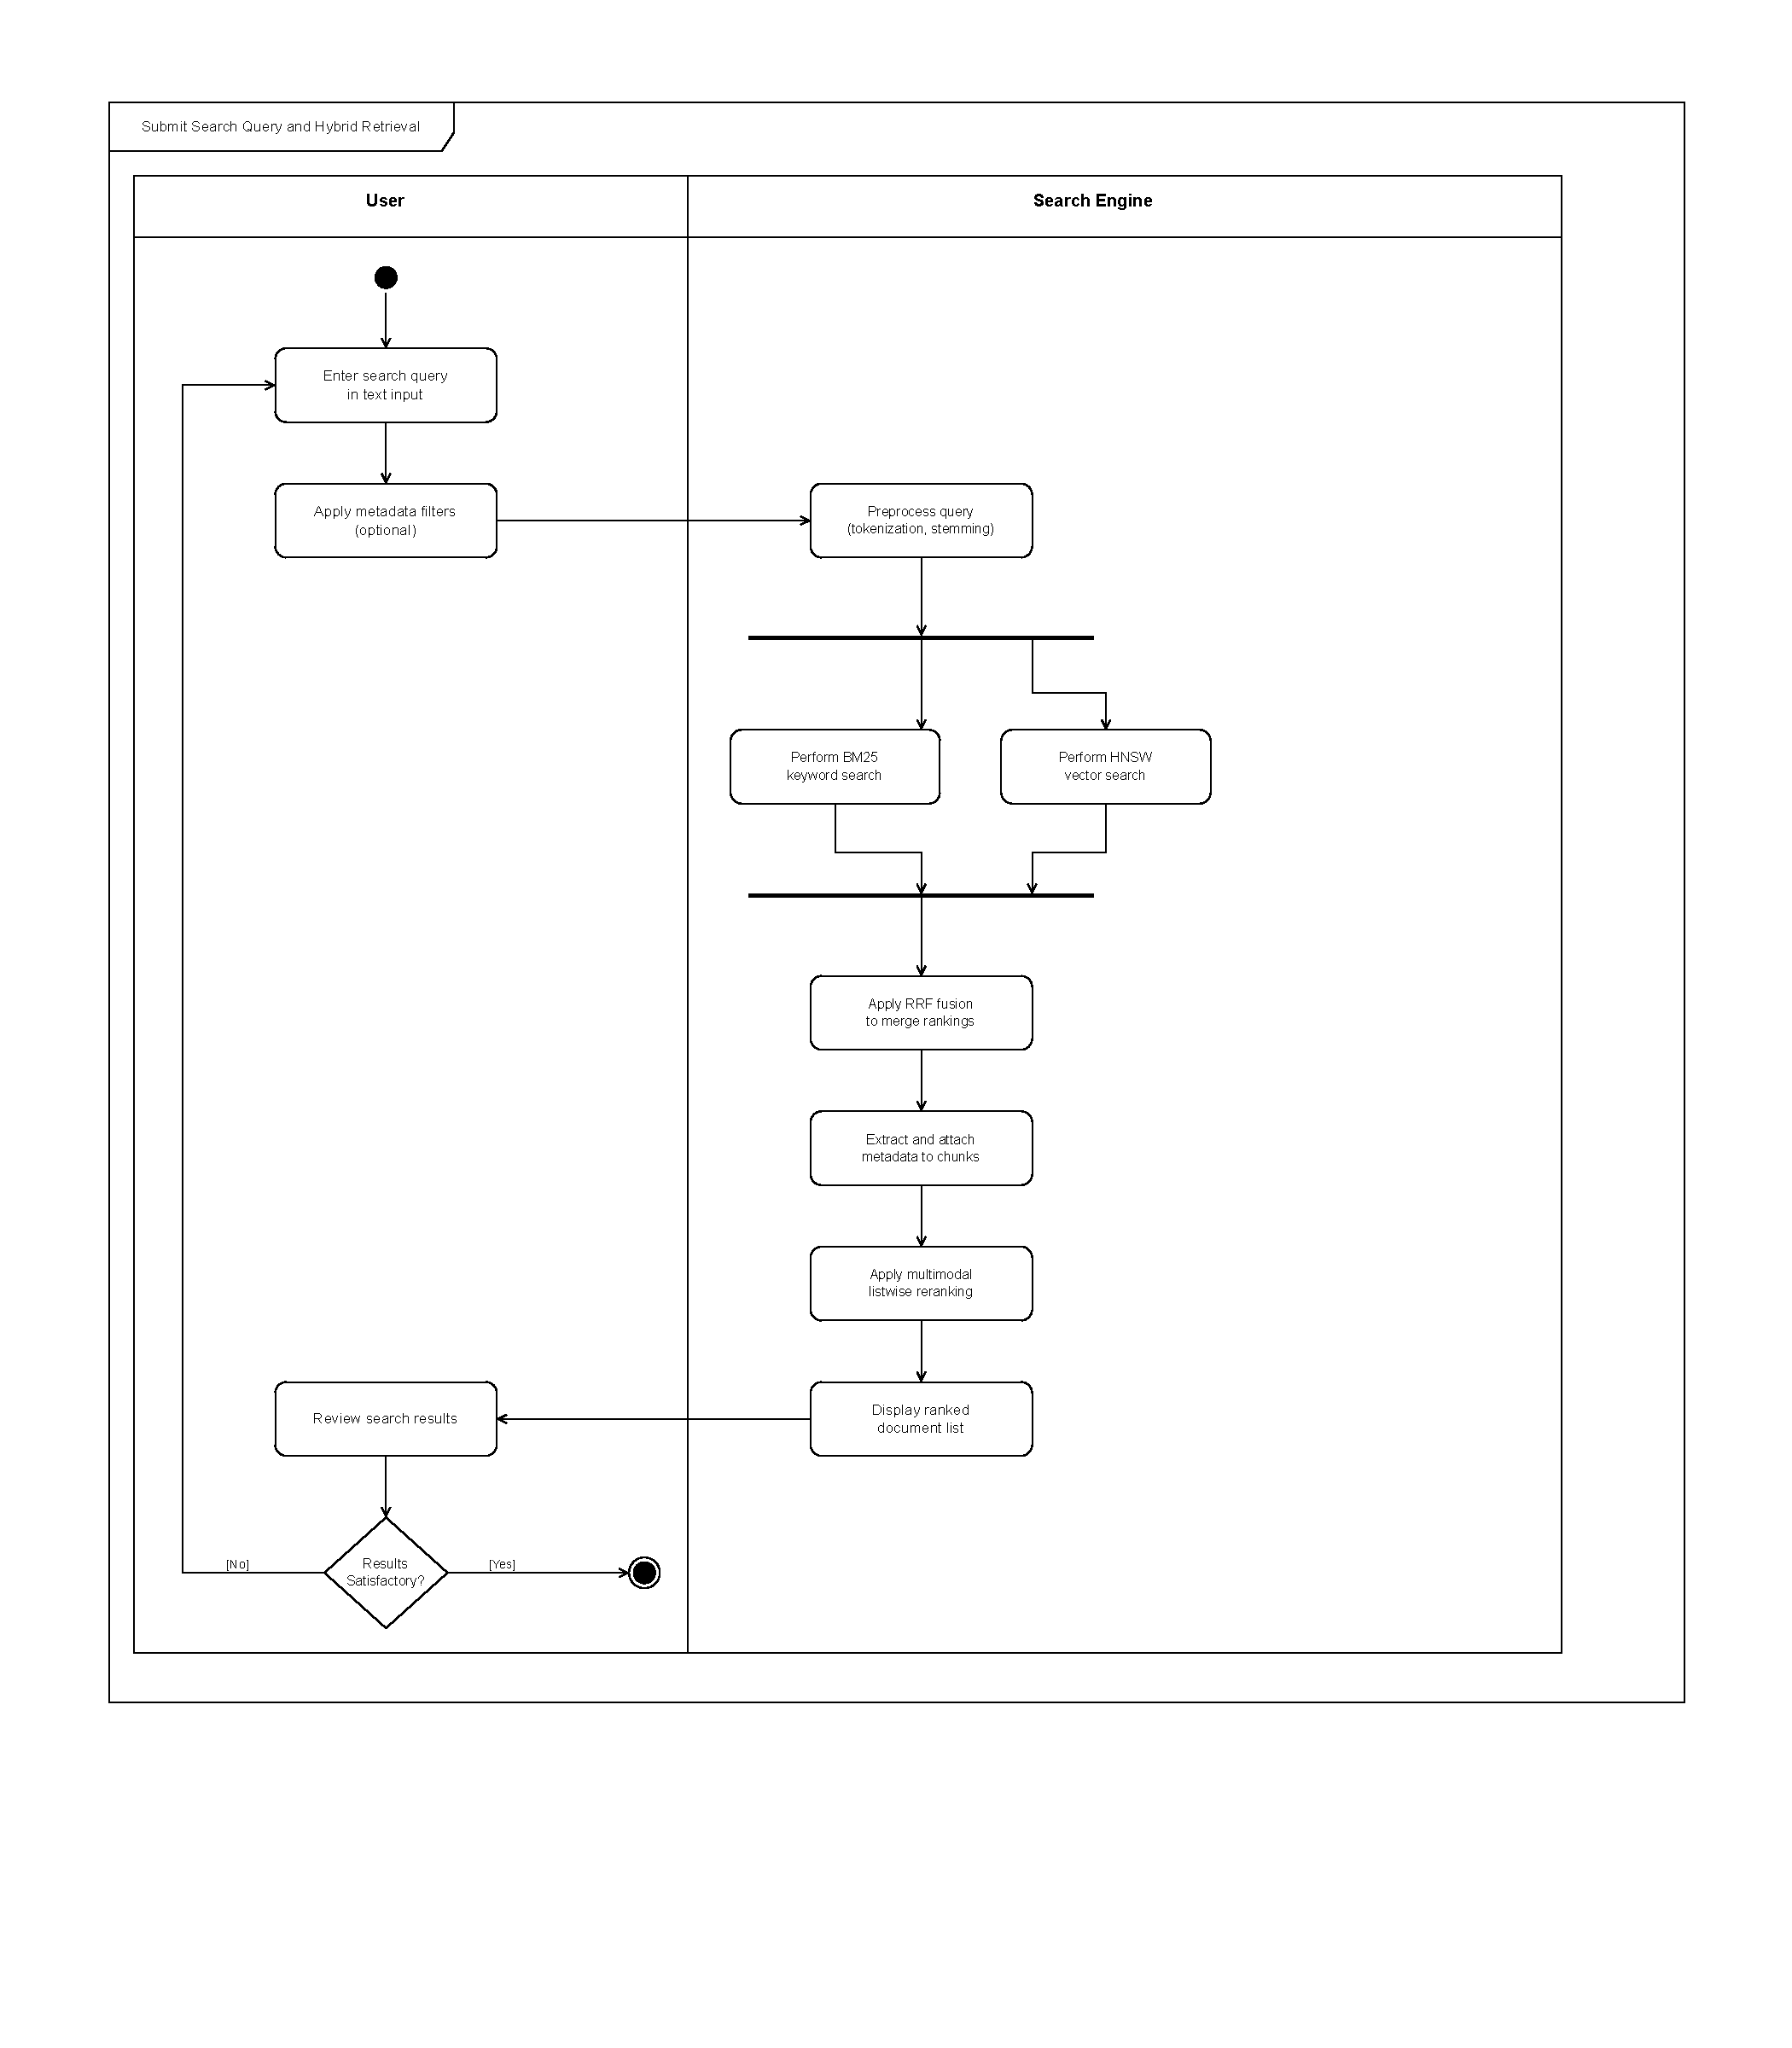
\includegraphics[width=0.55\linewidth]{activity3.drawio.pdf}
    \caption{Activity Diagram: Multimodal Reranking Process}
    \label{fig:activity3}
\end{figure}

Figure \ref{fig:activity3} details the multimodal reranking process using BLIP-2. After hybrid search produces top 20 candidates, the system retrieves associated images for each document. The reranker constructs a setwise prompt containing the query, document texts, and image references. BLIP-2's Q-Former architecture processes cross-modal interactions, encoding both textual semantics and visual content. The vision-language model evaluates each candidate's multimodal relevance, generating a reranked list that considers whether charts, diagrams, or other visual elements address the user's information need. This enables the system to properly rank technical documentation where critical information resides in visual components.

\begin{figure}[H]
    \centering
    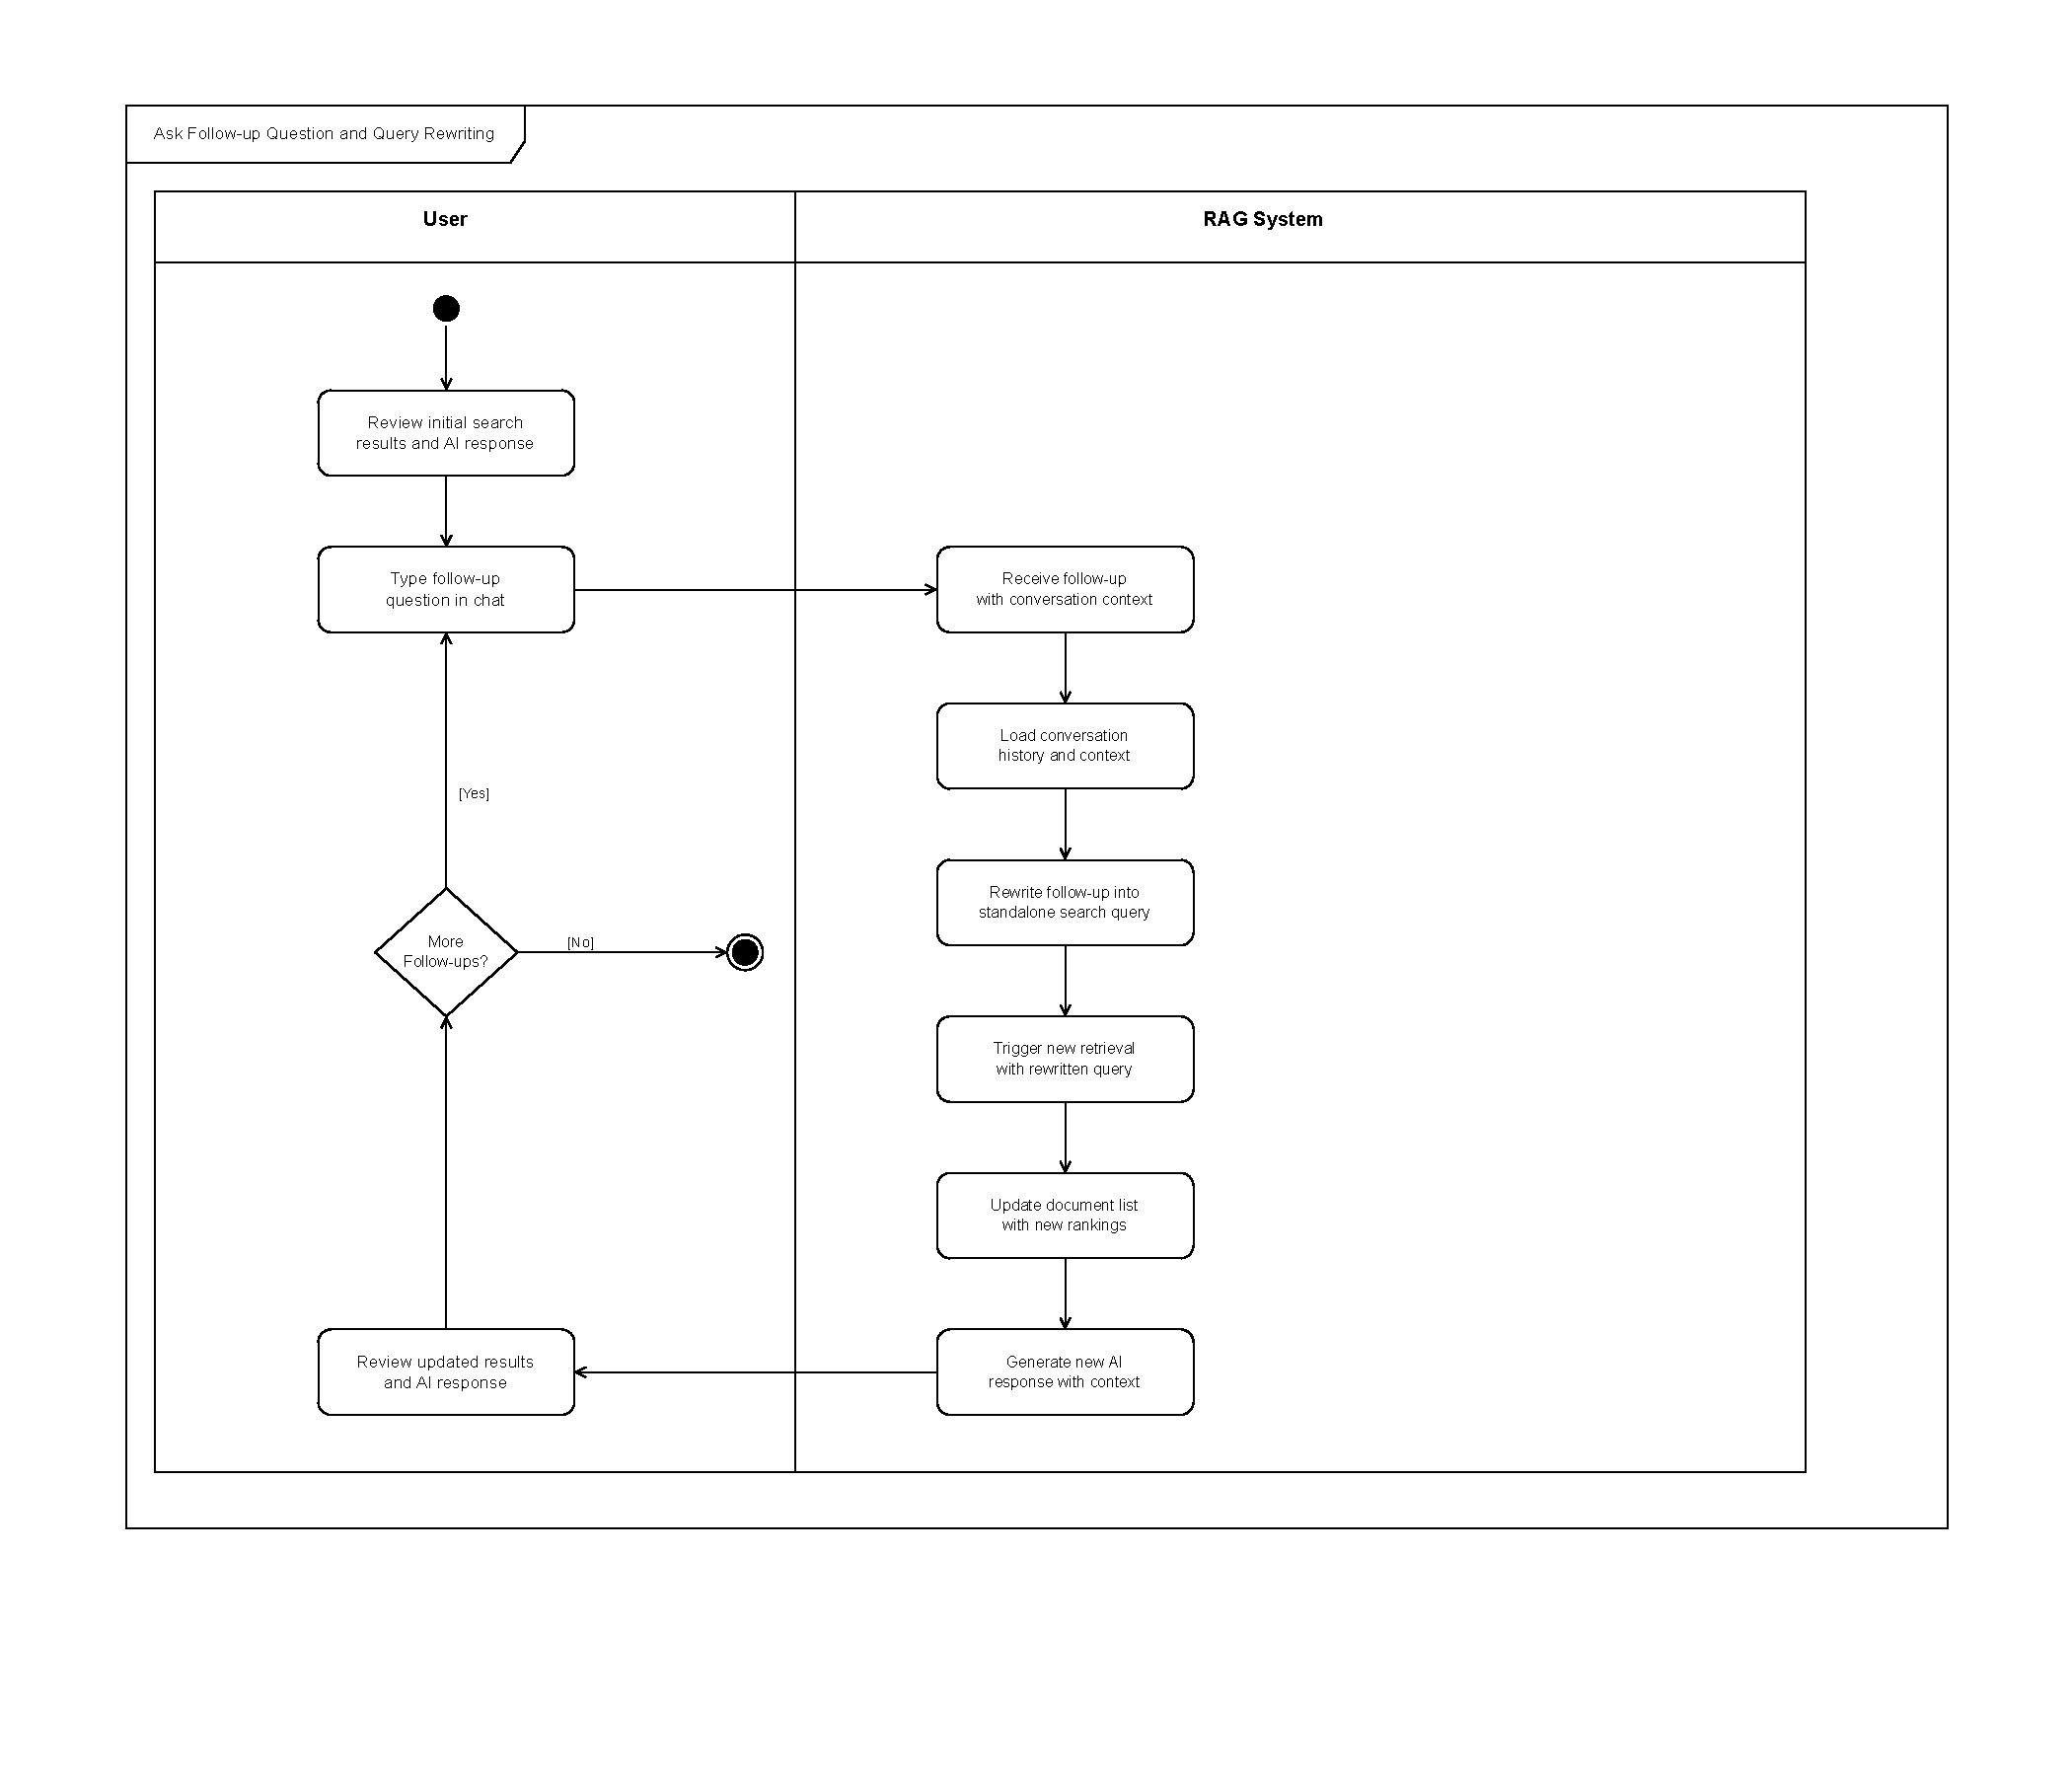
\includegraphics[width=0.55\linewidth]{activity4.drawio.pdf}
    \caption{Activity Diagram: Distributed Crawling Workflow}
    \label{fig:activity4}
\end{figure}

Figure \ref{fig:activity4} shows the distributed crawling coordination mechanism using Kafka. When an administrator triggers a crawl job, the coordinator partitions tasks across configured data sources (Confluence spaces, Google Drive folders, Git repositories, network shares). Tasks are published to the "crawl-tasks" Kafka topic, and worker nodes consume assignments based on availability. Each worker authenticates with its assigned source, recursively fetches documents while respecting rate limits, extracts text and images, and publishes results to the "documents-ingested" topic. Failed tasks trigger exponential backoff retries before being marked as failed. This architecture enables horizontal scaling by simply adding worker nodes to handle larger document collections.

\begin{figure}[H]
    \centering
    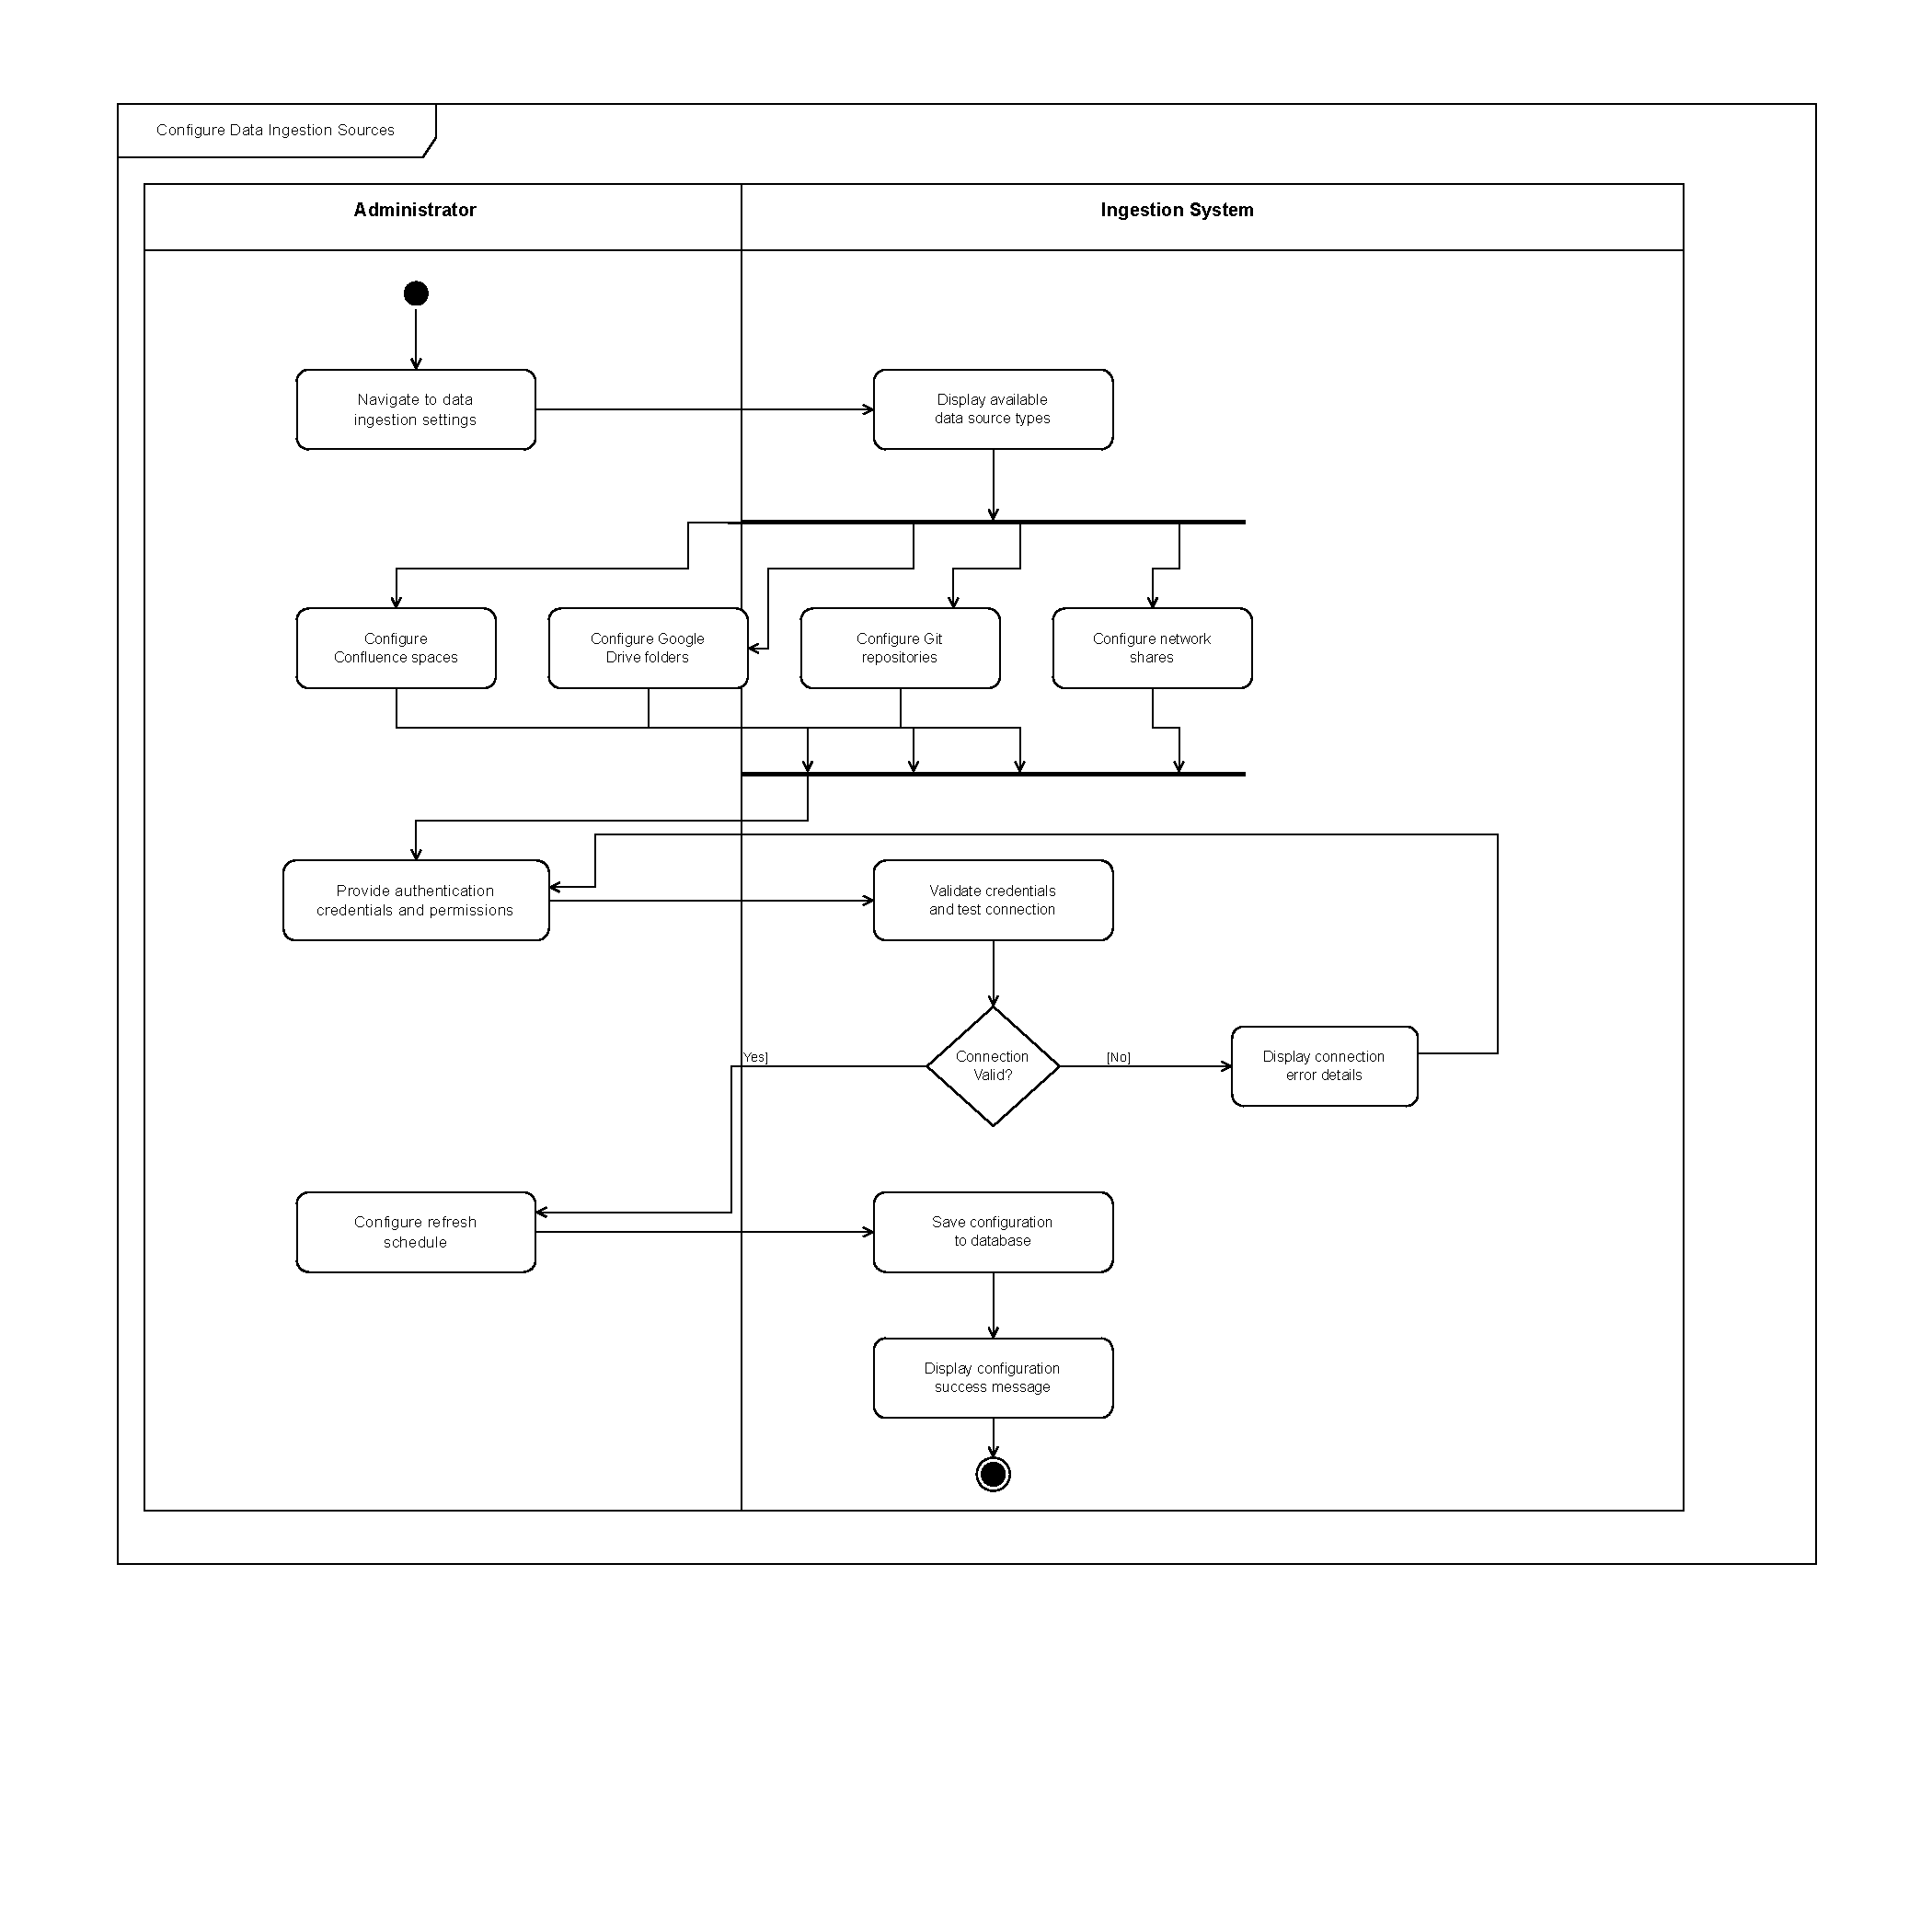
\includegraphics[width=0.55\linewidth]{activity5.drawio.pdf}
    \caption{Activity Diagram: Document Chunking and Embedding Generation}
    \label{fig:activity5}
\end{figure}

Figure \ref{fig:activity5} illustrates the document processing pipeline from ingestion to index building. Documents consumed from Kafka undergo format-specific extraction (PDF, DOCX, HTML) to separate text and images. The chunking module segments text into semantic units using heading structure, paragraph boundaries, or fixed token counts, maintaining 10\% overlap between adjacent chunks to preserve context. Text chunks are batched and encoded using Sentence-BERT on GPU, while images are processed through CLIP's vision encoder. Generated embeddings are inserted into the HNSW vector index, and document metadata is stored in PostgreSQL. This pipeline processes thousands of documents per hour using GPU acceleration and batch optimization.

\begin{figure}[H]
    \centering
    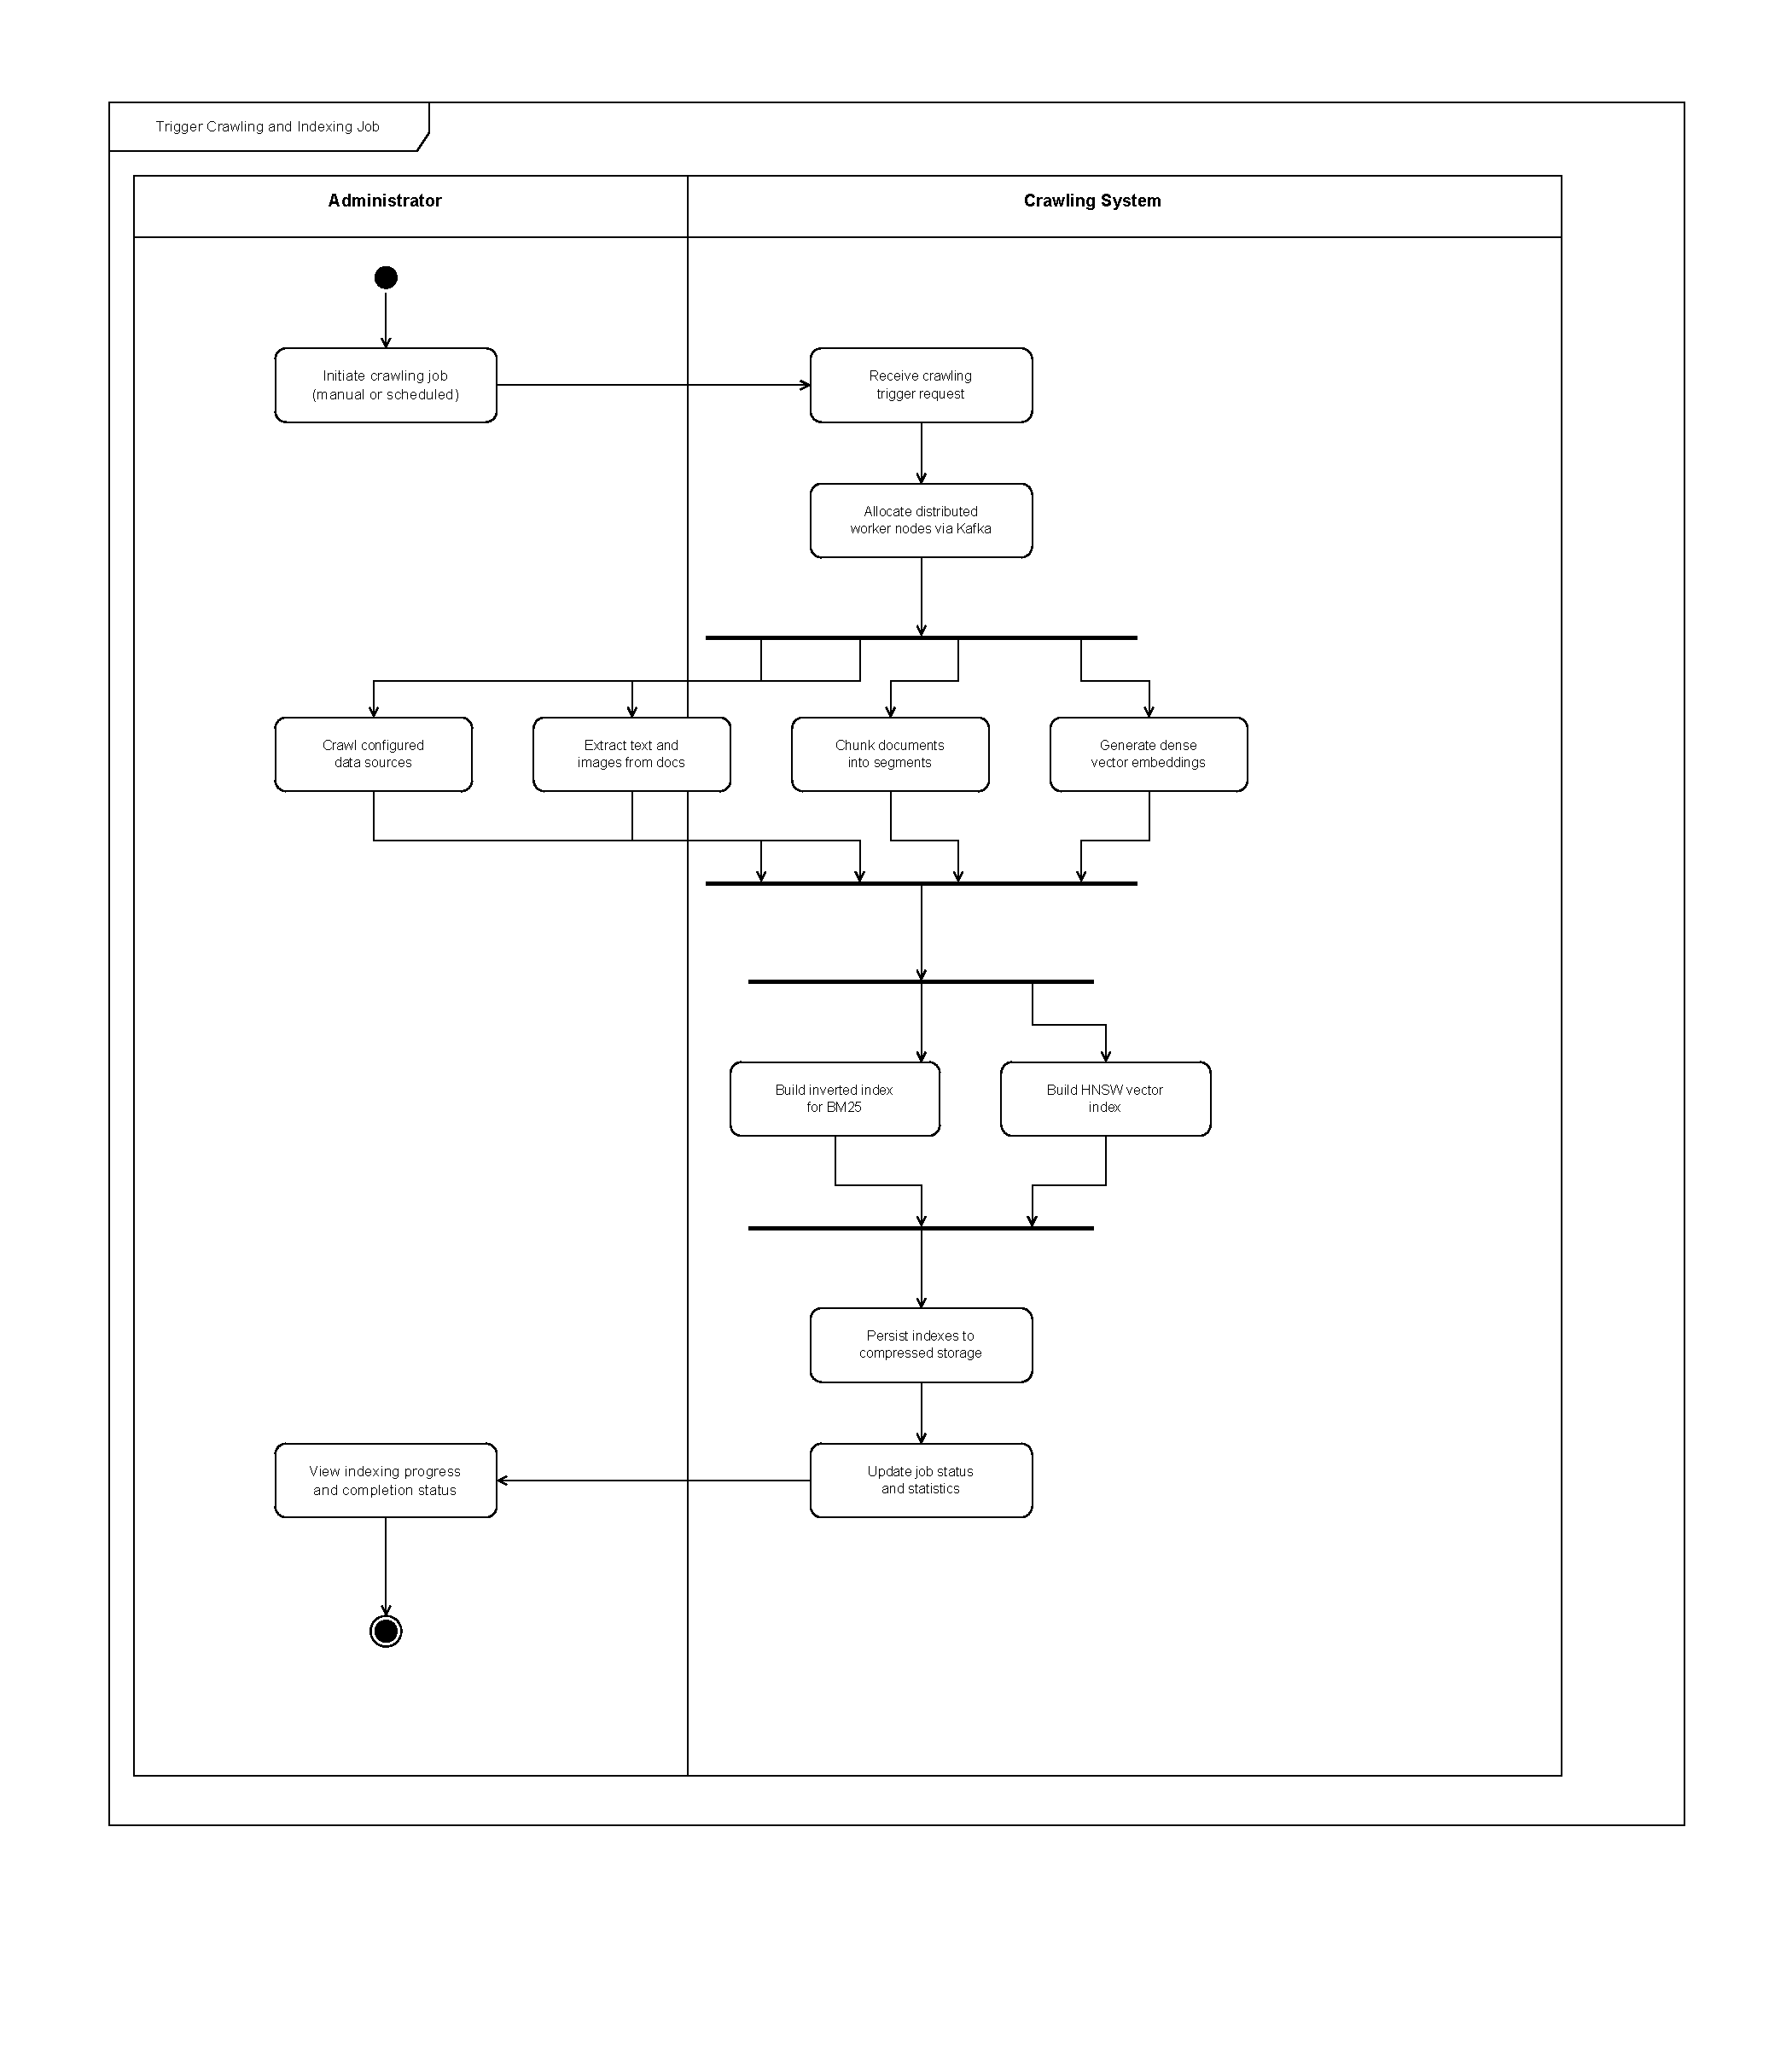
\includegraphics[width=0.55\linewidth]{activity6.drawio.pdf}
    \caption{Activity Diagram: RAG Answer Generation with Citations}
    \label{fig:activity6}
\end{figure}

Figure \ref{fig:activity6} depicts the retrieval-augmented generation workflow for producing grounded answers. Upon receiving a user query, the system executes the retrieval pipeline to fetch top K=5 most relevant chunks. These chunks are formatted into a structured prompt with clear delimiters and source identifiers. The system prompt explicitly instructs the LLM to answer based solely on provided context and to cite sources using [1], [2] notation. The LLM generates a response via SGLang, which streams tokens to the user interface in real-time. The system performs post-generation validation using an entailment model to verify claims against sources, flagging any unsupported assertions for review.

\begin{figure}[H]
    \centering
    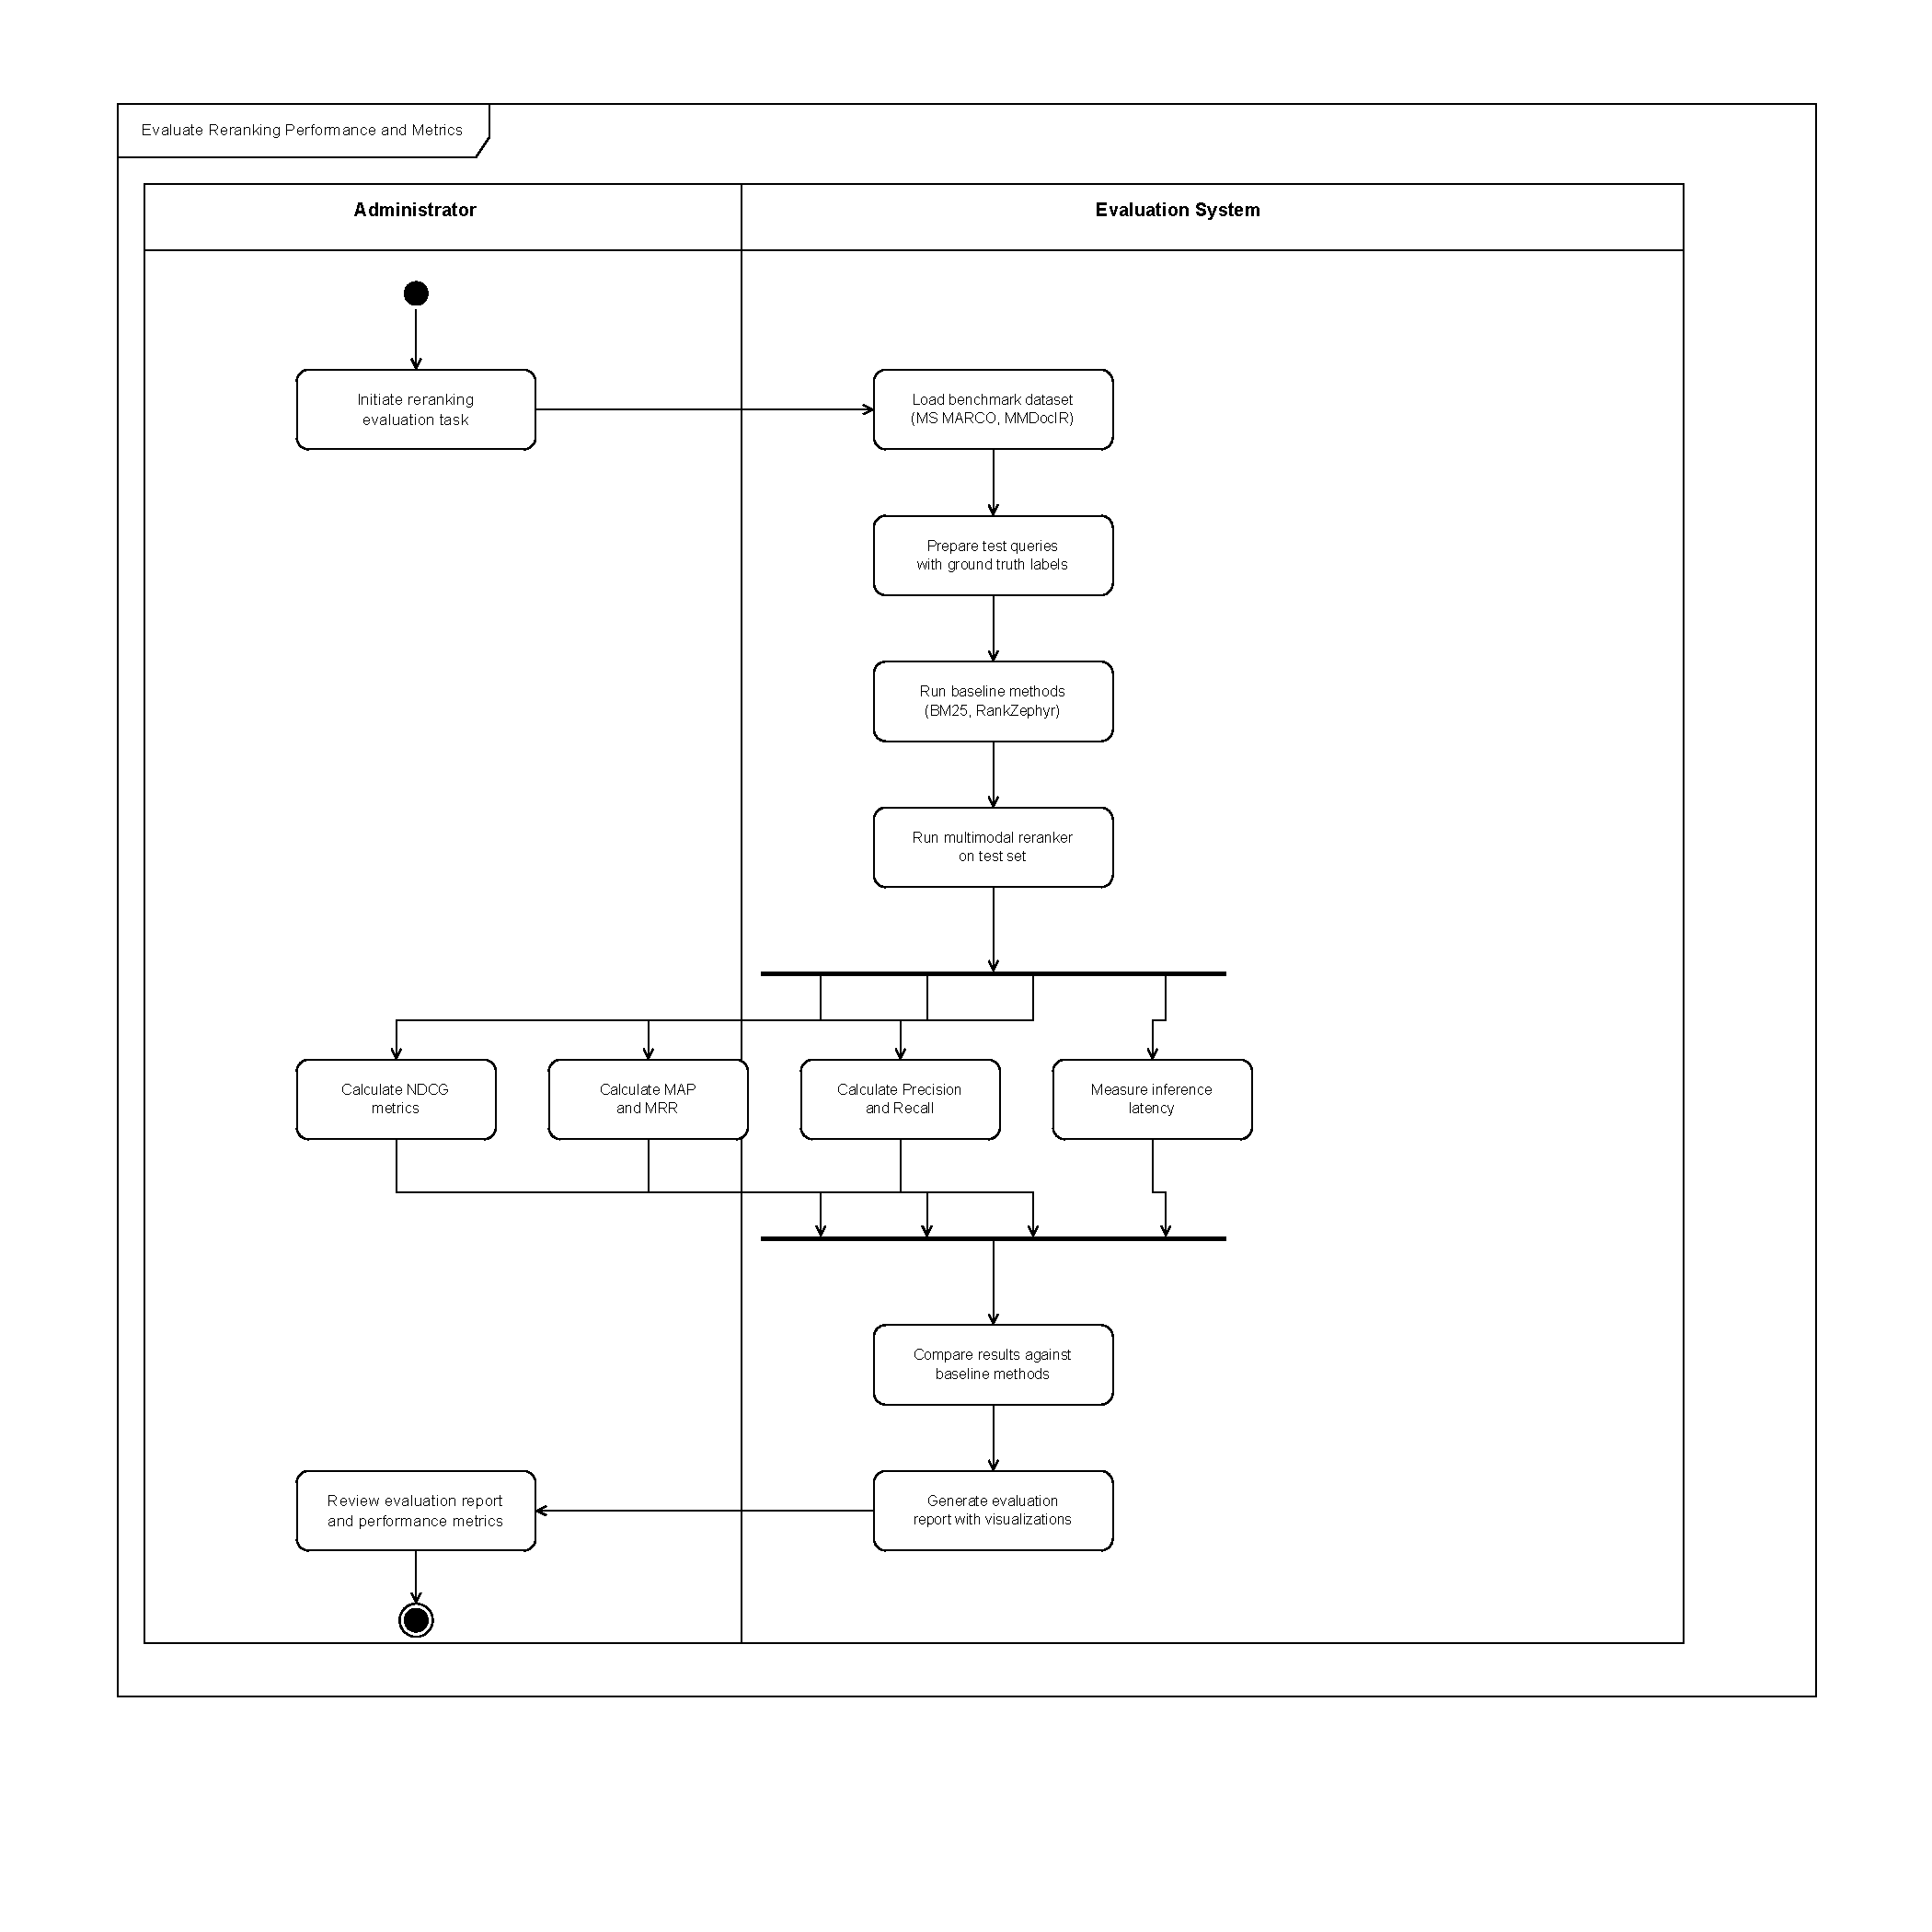
\includegraphics[width=0.55\linewidth]{activity7.drawio.pdf}
    \caption{Activity Diagram: Conversational Query Rewriting Flow}
    \label{fig:activity7}
\end{figure}

Figure \ref{fig:activity7} shows the conversational query rewriting mechanism that enables iterative search refinement. When the system detects a follow-up question (e.g., "What about performance optimization?"), it retrieves the last 10 conversation turns from Redis. These turns, along with the new query, are formatted into a rewriting prompt asking the LLM to produce a standalone query that captures the user's intent without requiring conversation context. The LLM generates the rewritten query, which triggers a new retrieval cycle. This closed-loop architecture allows the search system to continually improve results based on user interactions, creating an iterative exploration experience where each question builds upon previous findings.

\begin{figure}[H]
    \centering
    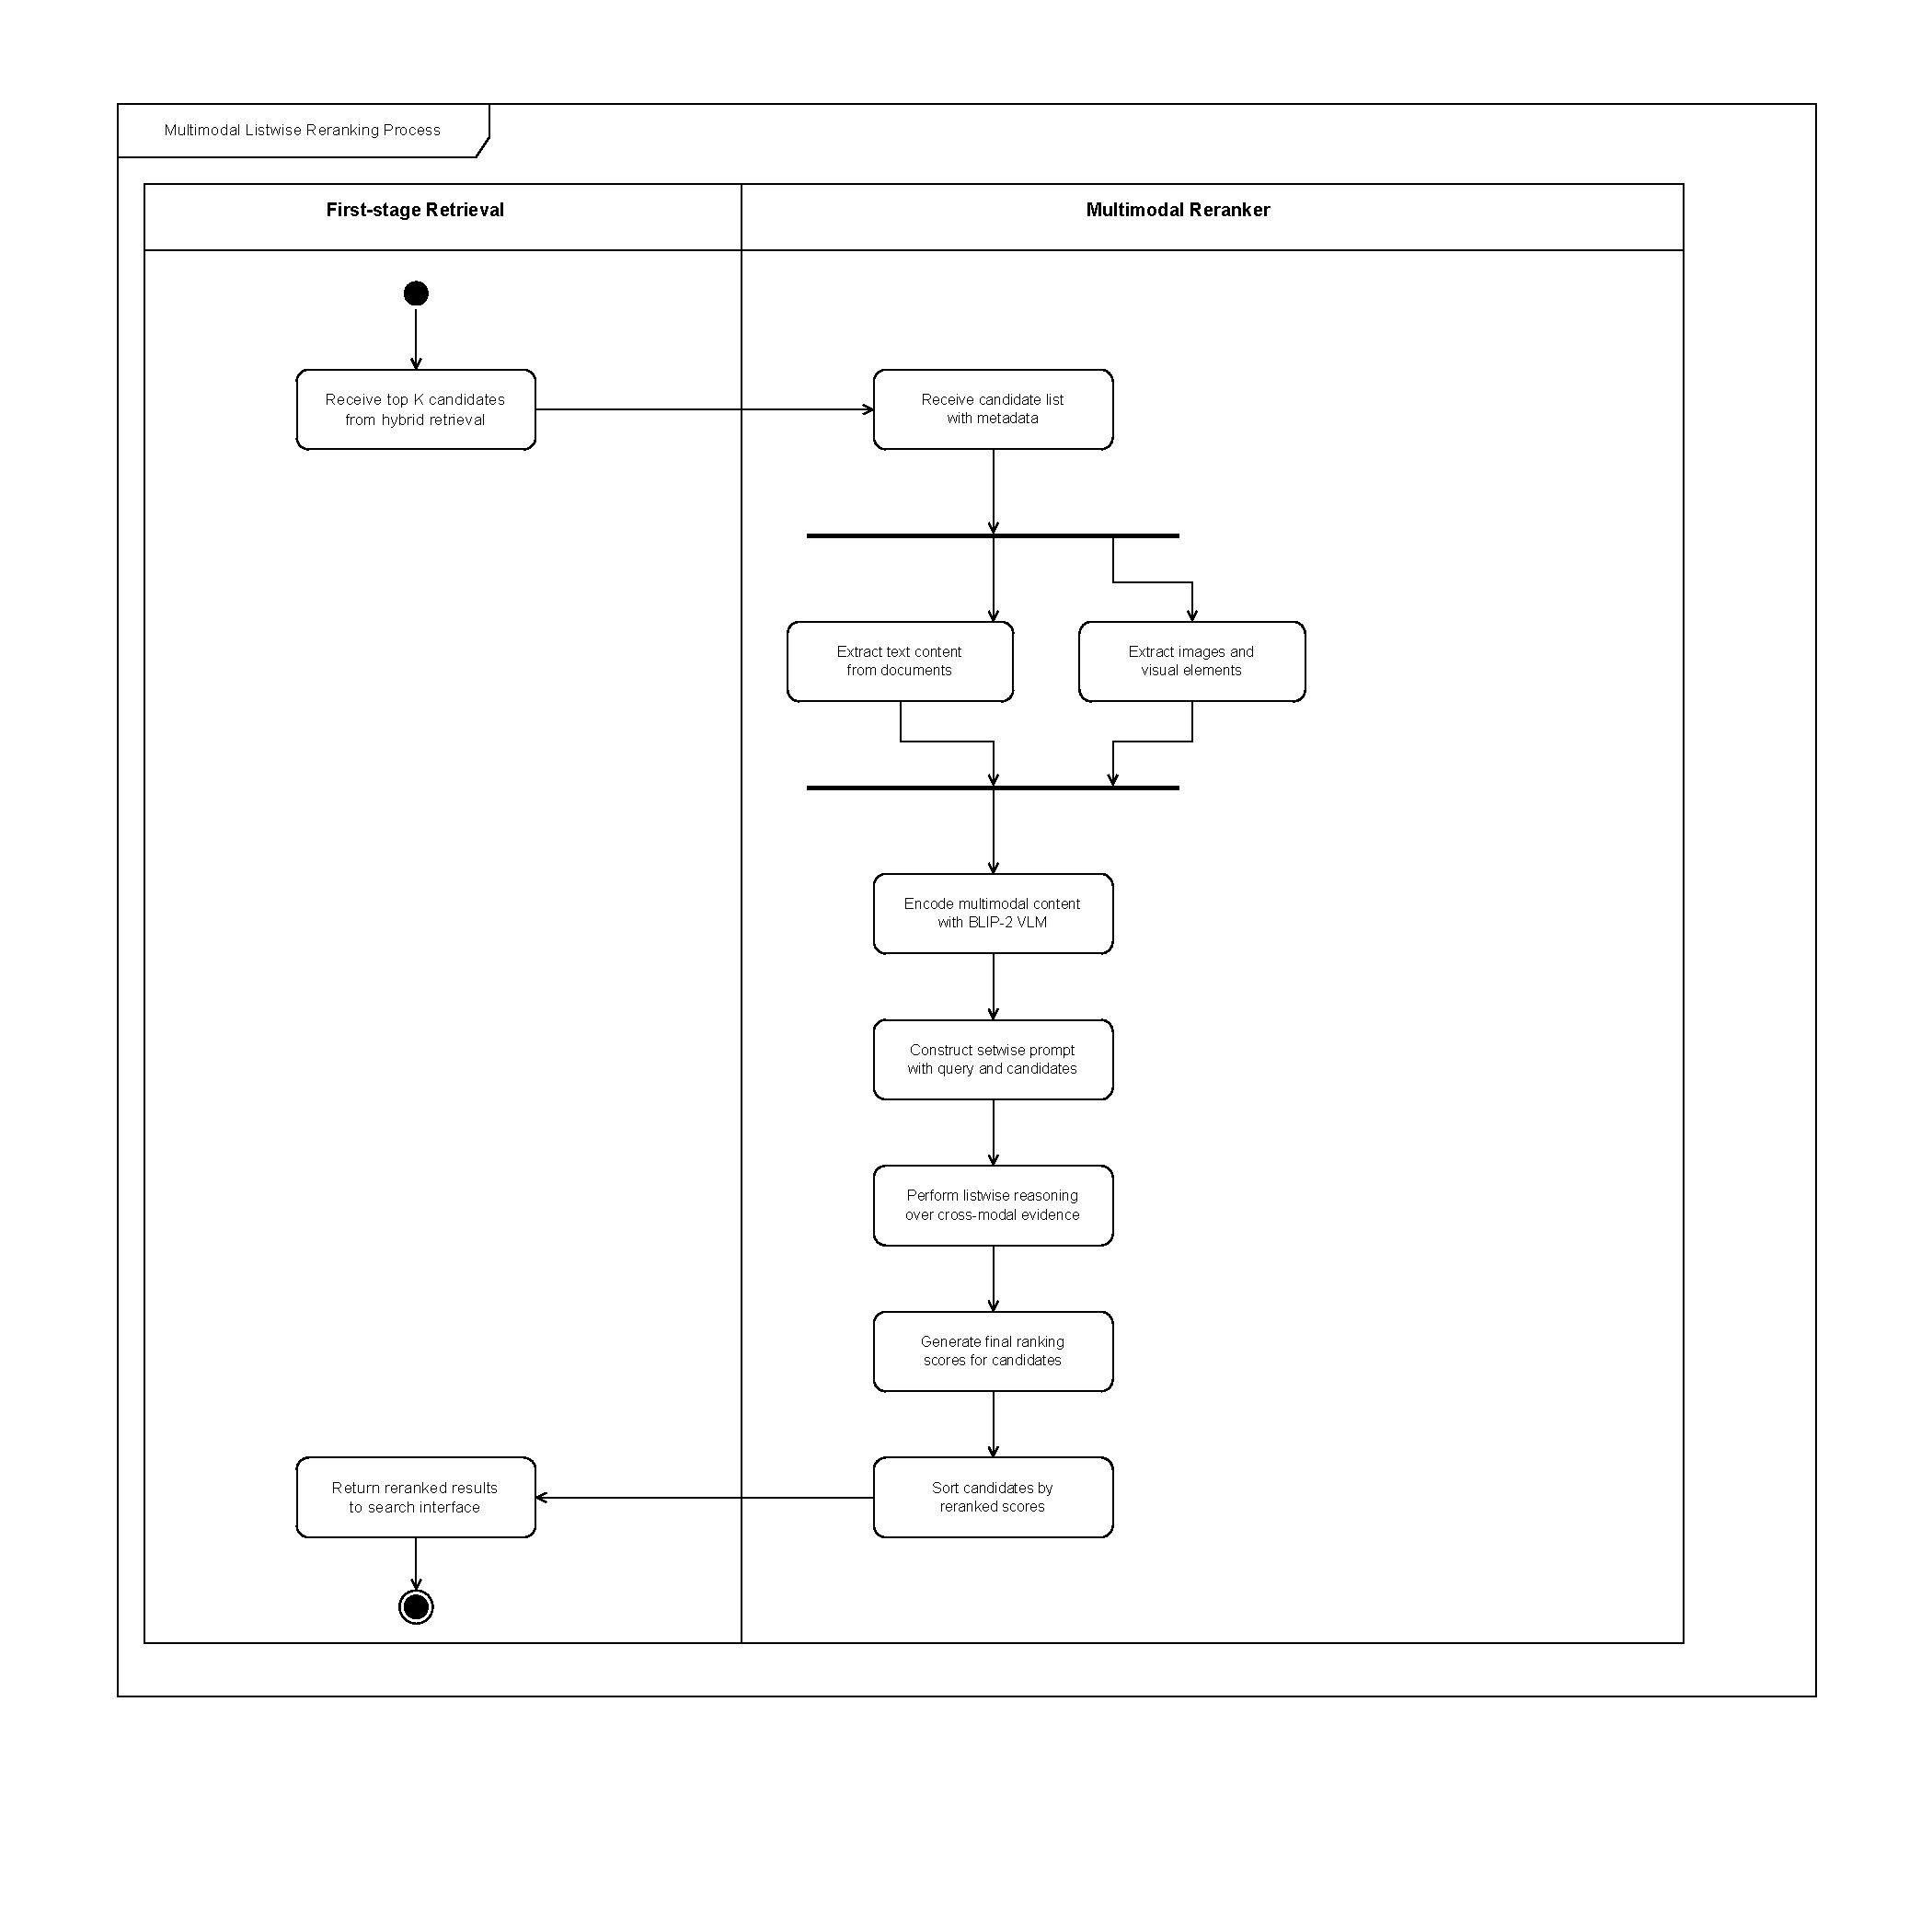
\includegraphics[width=0.55\linewidth]{activity8.drawio.pdf}
    \caption{Activity Diagram: Index Building and Refresh Process}
    \label{fig:activity8}
\end{figure}

Figure \ref{fig:activity8} illustrates the index building and refresh workflow. During initial indexing, the system processes all documents from configured sources, generating embeddings and building both inverted (BM25) and vector (HNSW) indices. For incremental updates, the system retrieves only documents modified since the last crawl timestamp, computes embeddings for new content, and merges them into existing indices using FAISS's add\_with\_ids method. The inverted index is updated by appending new term posting lists. After index updates complete, the system performs atomic swaps to replace the serving indices without downtime, ensuring continuous query availability. Index versions are tracked in PostgreSQL, enabling rollback if update issues arise.

\begin{figure}[H]
    \centering
    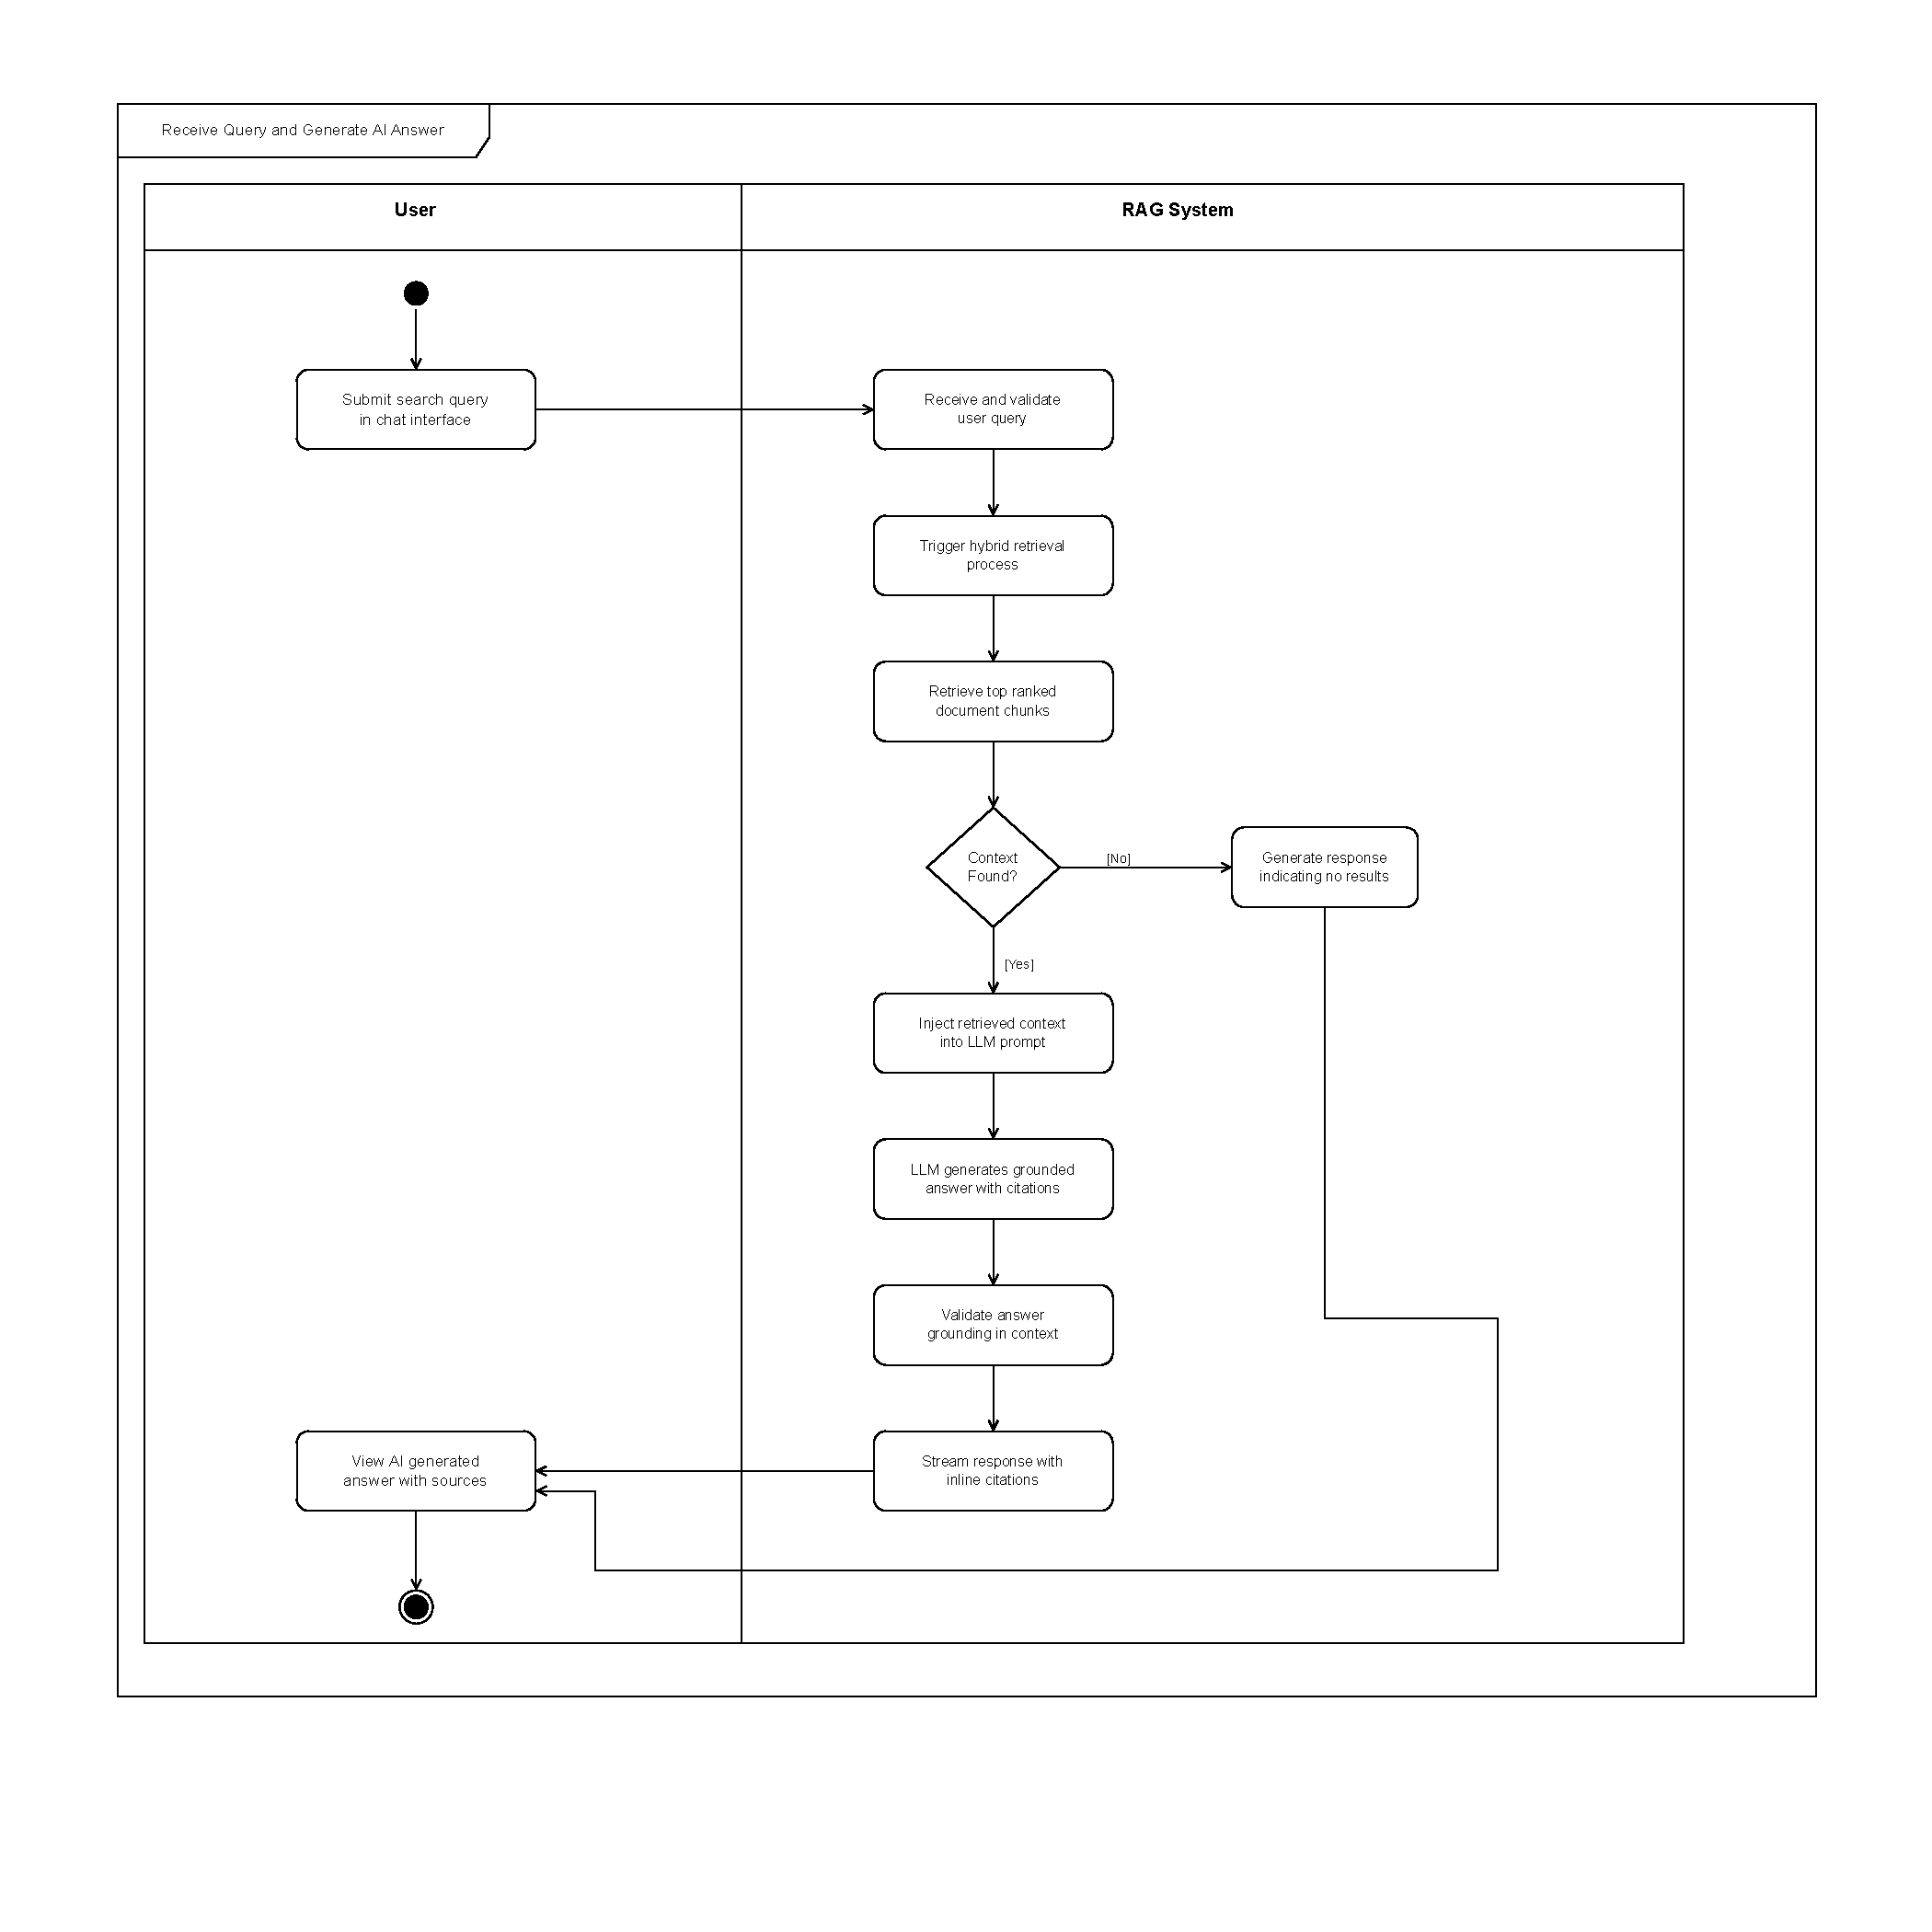
\includegraphics[width=0.55\linewidth]{activity9.drawio.pdf}
    \caption{Activity Diagram: Session Management and Access Control}
    \label{fig:activity9}
\end{figure}

Figure \ref{fig:activity9} details the session management and access control enforcement workflow. Upon successful authentication, the system generates a JWT token containing user ID, roles, and expiration timestamp (24 hours from issuance). This token is stored in a secure HTTP-only cookie to prevent XSS attacks. On each subsequent request, the system validates the JWT signature using the secret key, checks expiration, and extracts user information. When retrieving search results, the system enforces access control by filtering documents based on the user's permissions, querying PostgreSQL for the user's authorized document sets. This ensures users can only access documents they are permitted to view, maintaining data confidentiality across the enterprise.

\begin{figure}[H]
    \centering
    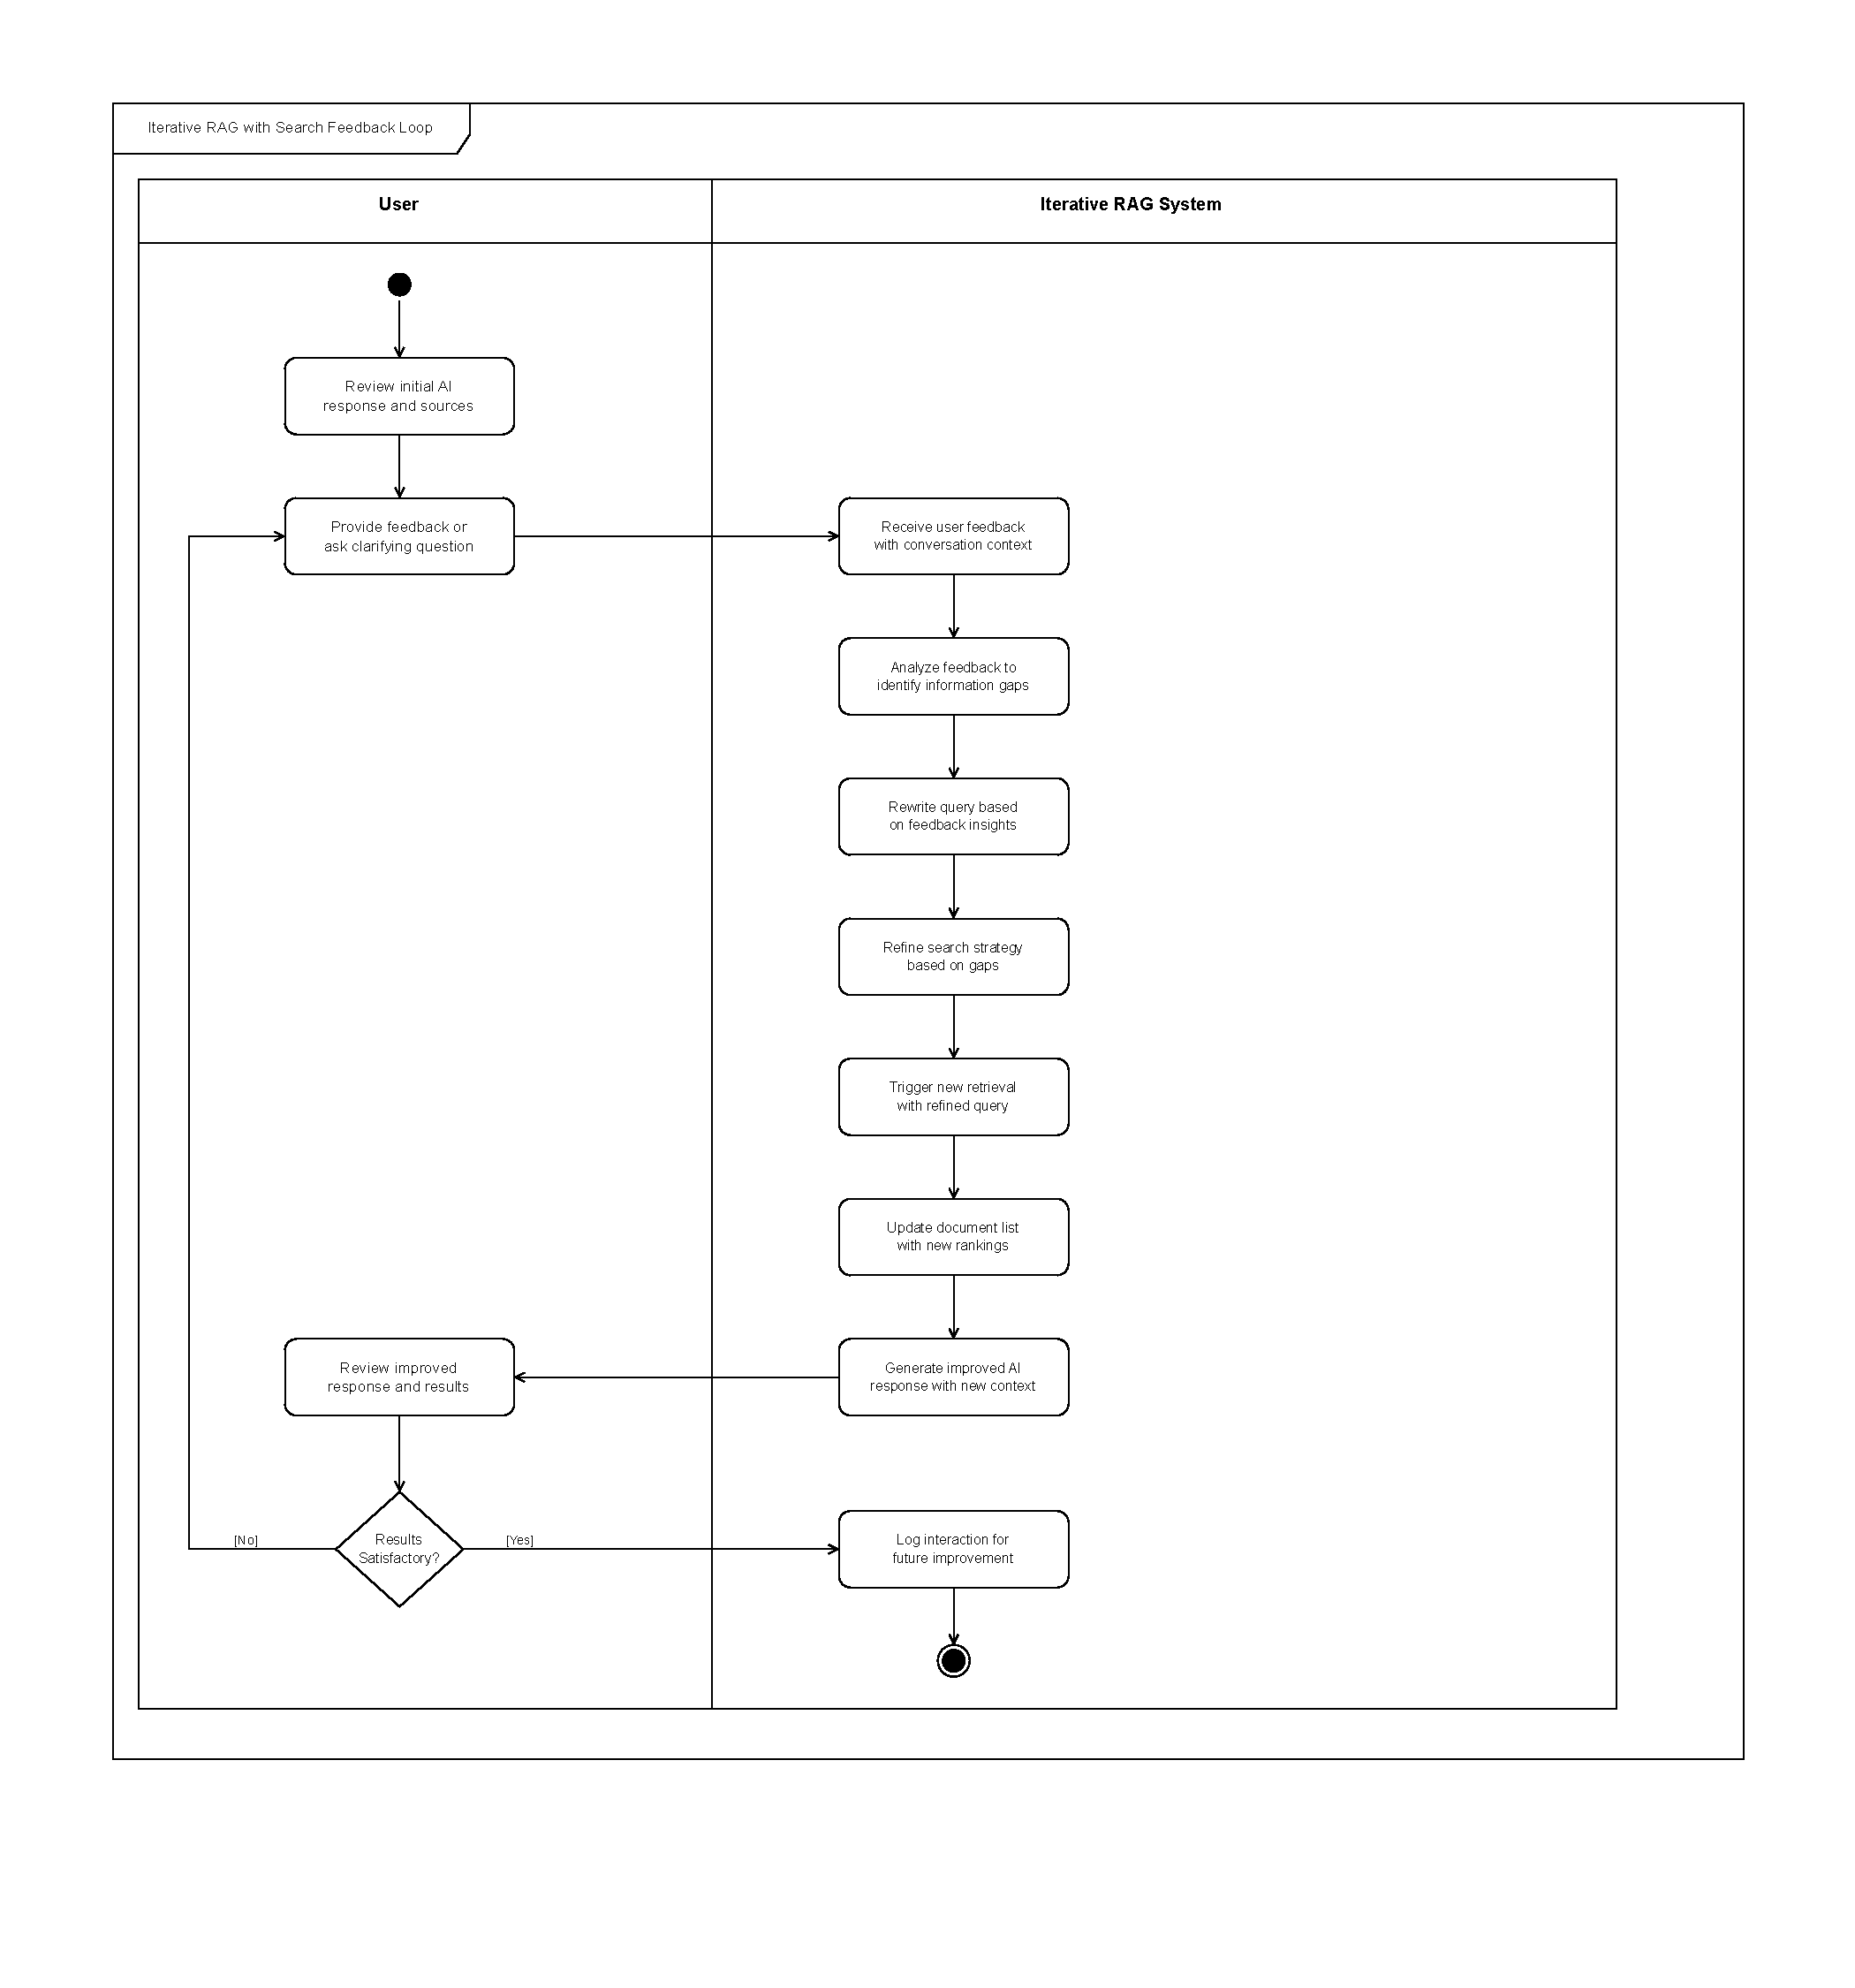
\includegraphics[width=0.55\linewidth]{activity10.drawio.pdf}
    \caption{Activity Diagram: Analytics and Monitoring Workflow}
    \label{fig:activity10}
\end{figure}

Figure \ref{fig:activity10} shows the analytics and monitoring system that tracks search quality and system performance. The system logs each search query with user ID, timestamp, query text, and result count. Query latency is measured at multiple stages (BM25 retrieval, vector search, reranking, total) and exported to Prometheus using histogram metrics. Click-through rates are tracked when users view documents from search results, providing implicit relevance feedback. Grafana dashboards visualize p90/p95/p99 latency distributions, query volume trends, and popular search terms. Alerting rules trigger notifications when latency exceeds 4 seconds or error rates exceed 1\%, enabling proactive performance optimization.

\clearpage


\section{Database Design}

This section presents the database schema for the Verdant Search system, designed using PostgreSQL to store user data, document metadata, search analytics, and system configuration. The database supports efficient query execution while maintaining data integrity through properly normalized tables and carefully designed indexes.

\begin{figure}[H]
    \centering
    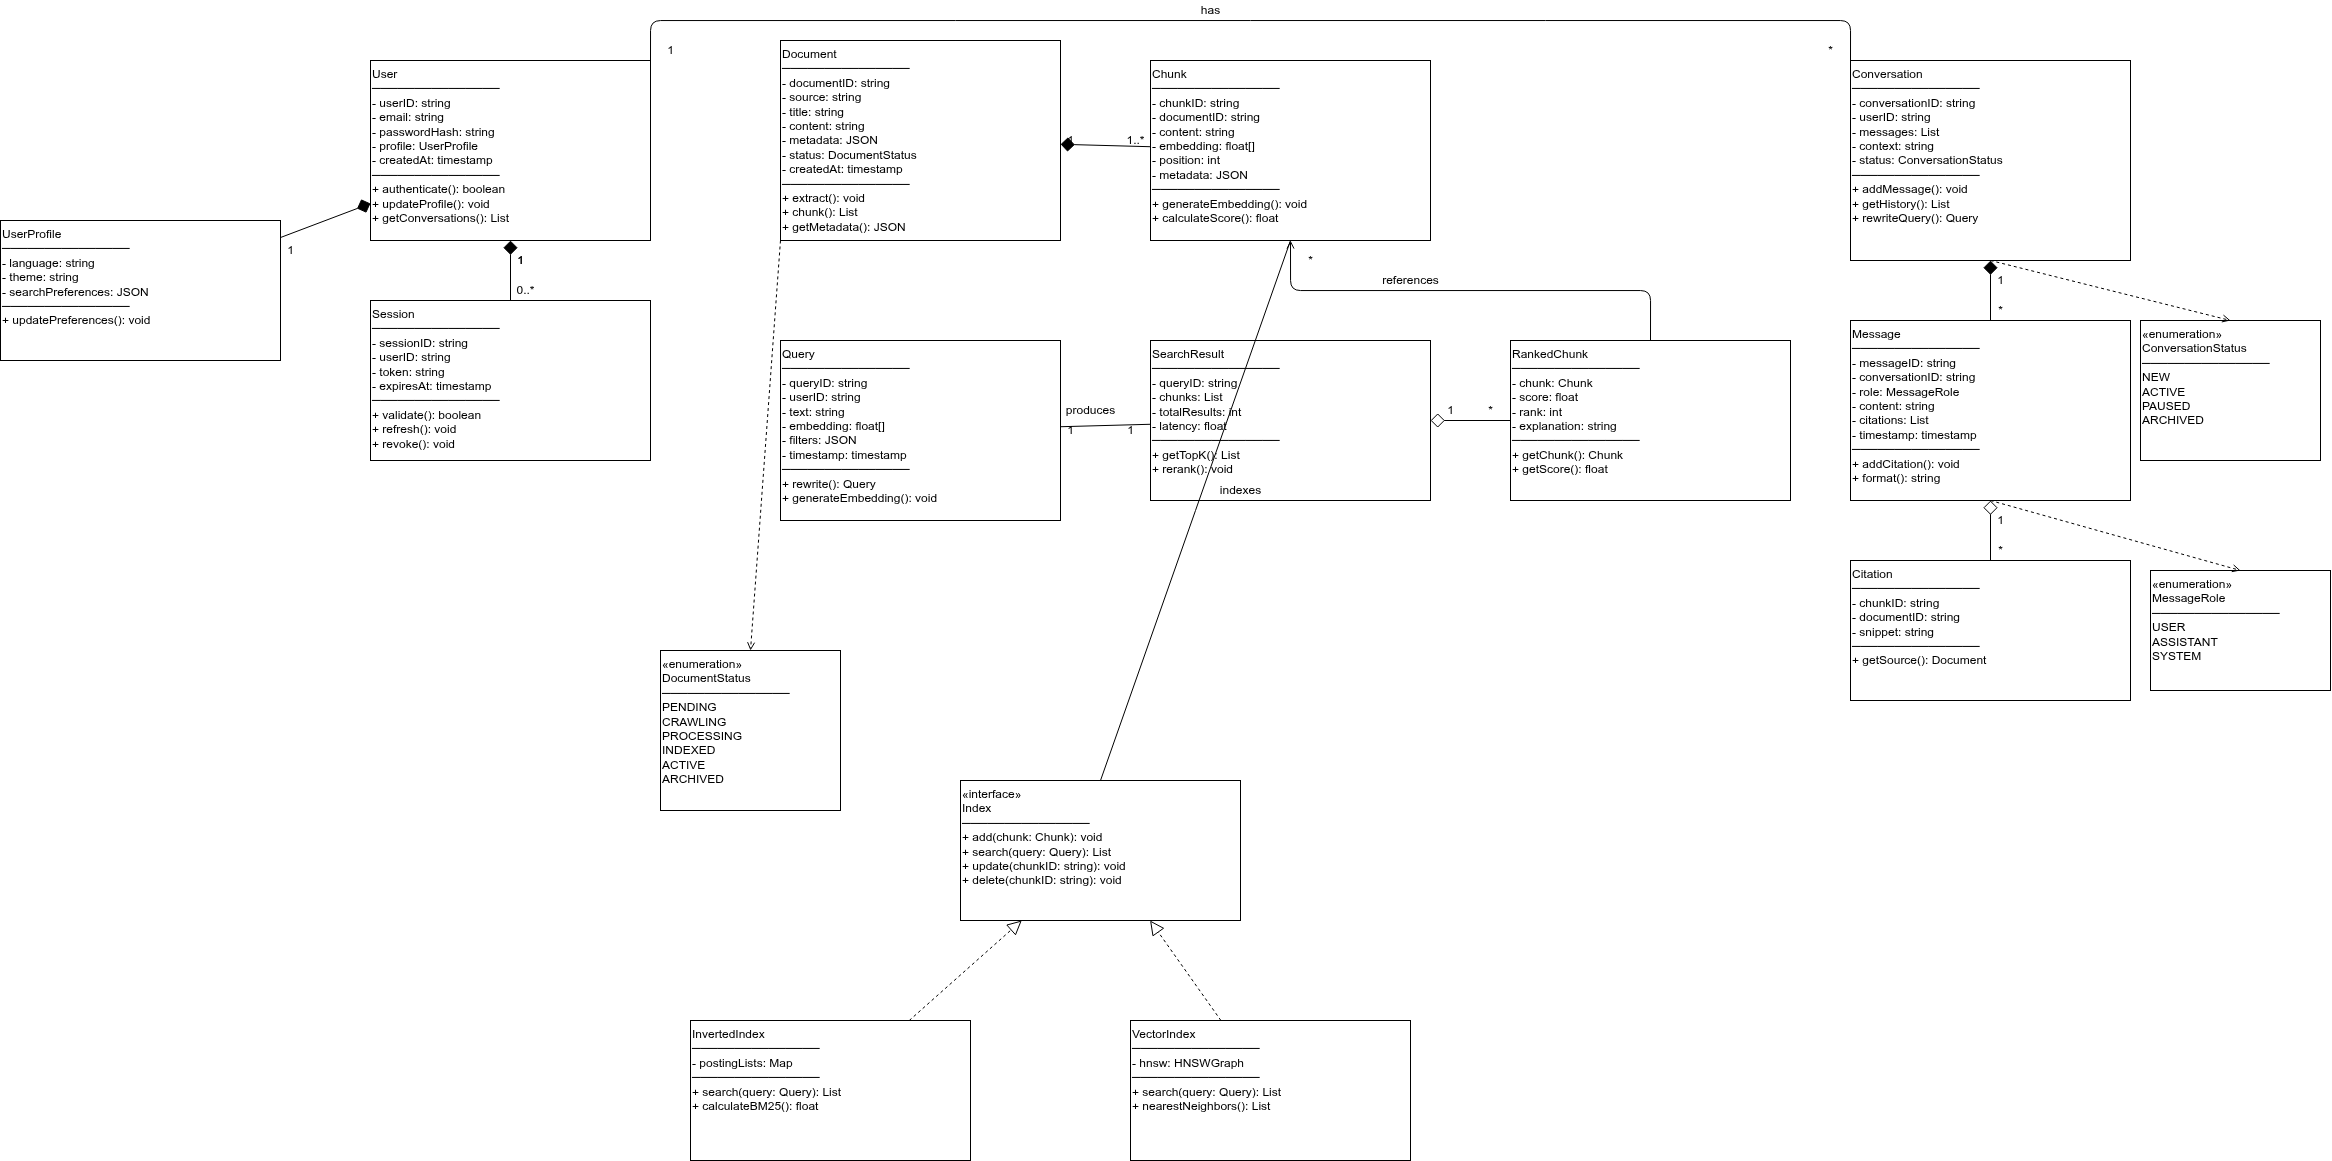
\includegraphics[width=\textwidth]{class.drawio.png}
    \caption{Entity-Relationship Diagram (Class Diagram Format) of Verdant Search Database}
    \label{fig:class_diagram}
\end{figure}

Figure \ref{fig:class_diagram} presents the complete database schema in class diagram notation. The design follows third normal form (3NF) to eliminate data redundancy while optimizing for common query patterns. Key entities and their relationships are described below:

\subsection{User Entity}
The \texttt{User} table stores authentication and profile information. Each user has a unique \texttt{user\_id} (UUID primary key), \texttt{email} (unique index for login lookups), \texttt{password\_hash} (bcrypt with cost factor 12), and optional SSO identifiers (\texttt{sso\_provider}, \texttt{sso\_id}). Profile fields include \texttt{display\_name}, \texttt{avatar\_url}, and \texttt{preferences} (JSONB for flexible settings). Timestamps track account \texttt{created\_at} and \texttt{last\_login}. The email column uses a unique B-tree index to enable fast authentication queries.

\subsection{Session Entity}
The \texttt{Session} table tracks active user sessions with JWT token management. Each session stores the \texttt{session\_id} (UUID), associated \texttt{user\_id} (foreign key to User), \texttt{token\_hash} (SHA-256 hash of JWT for revocation), \texttt{created\_at}, and \texttt{expires\_at} timestamps. An index on \texttt{user\_id} enables efficient retrieval of all sessions for a user. The system periodically purges expired sessions using a background job that deletes rows where \texttt{expires\_at < NOW()}.

\subsection{Document Entity}
The \texttt{Document} table contains metadata for all indexed documents. Core fields include \texttt{document\_id} (UUID), \texttt{title}, \texttt{content\_hash} (SHA-256 for deduplication), \texttt{source\_type} (enum: Confluence, GoogleDrive, Git, NetworkShare), \texttt{source\_url} (original location), \texttt{file\_type} (MIME type), \texttt{file\_size\_bytes}, and storage paths (\texttt{text\_storage\_path}, \texttt{images\_storage\_path}). Timestamps include \texttt{created\_at}, \texttt{modified\_at}, and \texttt{indexed\_at}. A GiN index on \texttt{source\_type} accelerates filtering queries.

\subsection{DocumentChunk Entity}
The \texttt{DocumentChunk} table stores segmented document portions for retrieval. Each chunk has \texttt{chunk\_id} (UUID), parent \texttt{document\_id} (foreign key), \texttt{chunk\_index} (integer position within document), \texttt{text\_content} (up to 2048 characters), \texttt{embedding\_id} (reference to vector index), and \texttt{token\_count}. The compound index on (\texttt{document\_id}, \texttt{chunk\_index}) enables efficient retrieval of all chunks for a document in sequential order.

\subsection{ConversationHistory Entity}
The \texttt{ConversationHistory} table tracks user chat sessions for RAG. Each entry stores \texttt{conversation\_id} (UUID), \texttt{user\_id} (foreign key), \texttt{message\_index} (sequence number), \texttt{role} (enum: user, assistant, system), \texttt{message\_content} (TEXT), and \texttt{timestamp}. An index on (\texttt{user\_id}, \texttt{timestamp} DESC) enables fast retrieval of recent conversation history for query rewriting. The system retains only the last 10 turns per user by periodically deleting older messages.

\subsection{SearchQuery Entity}
The \texttt{SearchQuery} table logs all search queries for analytics. Fields include \texttt{query\_id} (UUID), \texttt{user\_id} (foreign key), \texttt{query\_text}, \texttt{result\_count}, latency metrics (\texttt{bm25\_latency\_ms}, \texttt{vector\_latency\_ms}, \texttt{rerank\_latency\_ms}, \texttt{total\_latency\_ms}), and \texttt{timestamp}. Indexes on \texttt{user\_id} and \texttt{timestamp} support both user-specific query history views and time-series analytics. This table feeds Grafana dashboards for performance monitoring.

\subsection{SearchResult Entity}
The \texttt{SearchResult} table tracks which documents were returned for each query. It links \texttt{query\_id} to \texttt{document\_id} with additional fields for \texttt{rank\_position}, \texttt{relevance\_score}, and \texttt{was\_clicked} (boolean indicating user interaction). This enables click-through rate analysis to measure search quality. The compound index on (\texttt{query\_id}, \texttt{rank\_position}) supports efficient result retrieval.

\subsection{DataSource Entity}
The \texttt{DataSource} table stores configuration for crawl sources. Each source has \texttt{source\_id} (UUID), \texttt{source\_type} (enum matching Document source types), \texttt{connection\_url}, encrypted \texttt{credentials} (AES-256), \texttt{crawl\_schedule} (cron expression), \texttt{last\_crawl\_at}, and \texttt{is\_active} flag. The system decrypts credentials at crawl time using a master key stored in environment variables, never persisting plaintext credentials.

\subsection{CrawlJob Entity}
The \texttt{CrawlJob} table tracks distributed crawling execution. Each job records \texttt{job\_id} (UUID), \texttt{source\_id} (foreign key), \texttt{status} (enum: queued, running, completed, failed), \texttt{started\_at}, \texttt{completed\_at}, progress counters (\texttt{documents\_processed}, \texttt{documents\_failed}), and \texttt{error\_message} if failed. Indexes on \texttt{source\_id} and \texttt{status} enable monitoring dashboard queries.

\subsection{AccessControl Entity}
The \texttt{AccessControl} table implements document permission management. It creates a many-to-many relationship between Users and Documents through entries containing \texttt{user\_id}, \texttt{document\_id}, and \texttt{permission\_level} (enum: read, write, admin). A compound unique index on (\texttt{user\_id}, \texttt{document\_id}) prevents duplicate permission entries. Search queries join this table to filter results based on the requesting user's permissions, enforcing enterprise access control policies.

\subsection{Key Indexes and Performance Optimizations}

The database schema includes carefully designed indexes to support common query patterns:

\begin{itemize}
    \item \textbf{User.email (B-tree unique):} Enables fast login credential lookups with O(log n) complexity.
    \item \textbf{Document.source\_type (GIN):} Accelerates filtering by data source type for source-specific queries.
    \item \textbf{DocumentChunk.(document\_id, chunk\_index) (composite B-tree):} Enables efficient sequential chunk retrieval for RAG context assembly.
    \item \textbf{ConversationHistory.(user\_id, timestamp DESC) (composite B-tree):} Supports fast retrieval of recent conversation history for query rewriting.
    \item \textbf{SearchQuery.timestamp (B-tree):} Enables time-series analytics queries for Grafana dashboards.
    \item \textbf{AccessControl.(user\_id, document\_id) (unique composite):} Ensures unique permissions and accelerates access control checks during search.
\end{itemize}

All tables use UUID primary keys to enable distributed database scaling and prevent ID collision. Foreign key constraints enforce referential integrity, with CASCADE deletes configured where appropriate (e.g., deleting a User cascades to their Sessions and ConversationHistory).

\clearpage


\section{Deployment Architecture}

\begin{figure}[H]
    \centering
    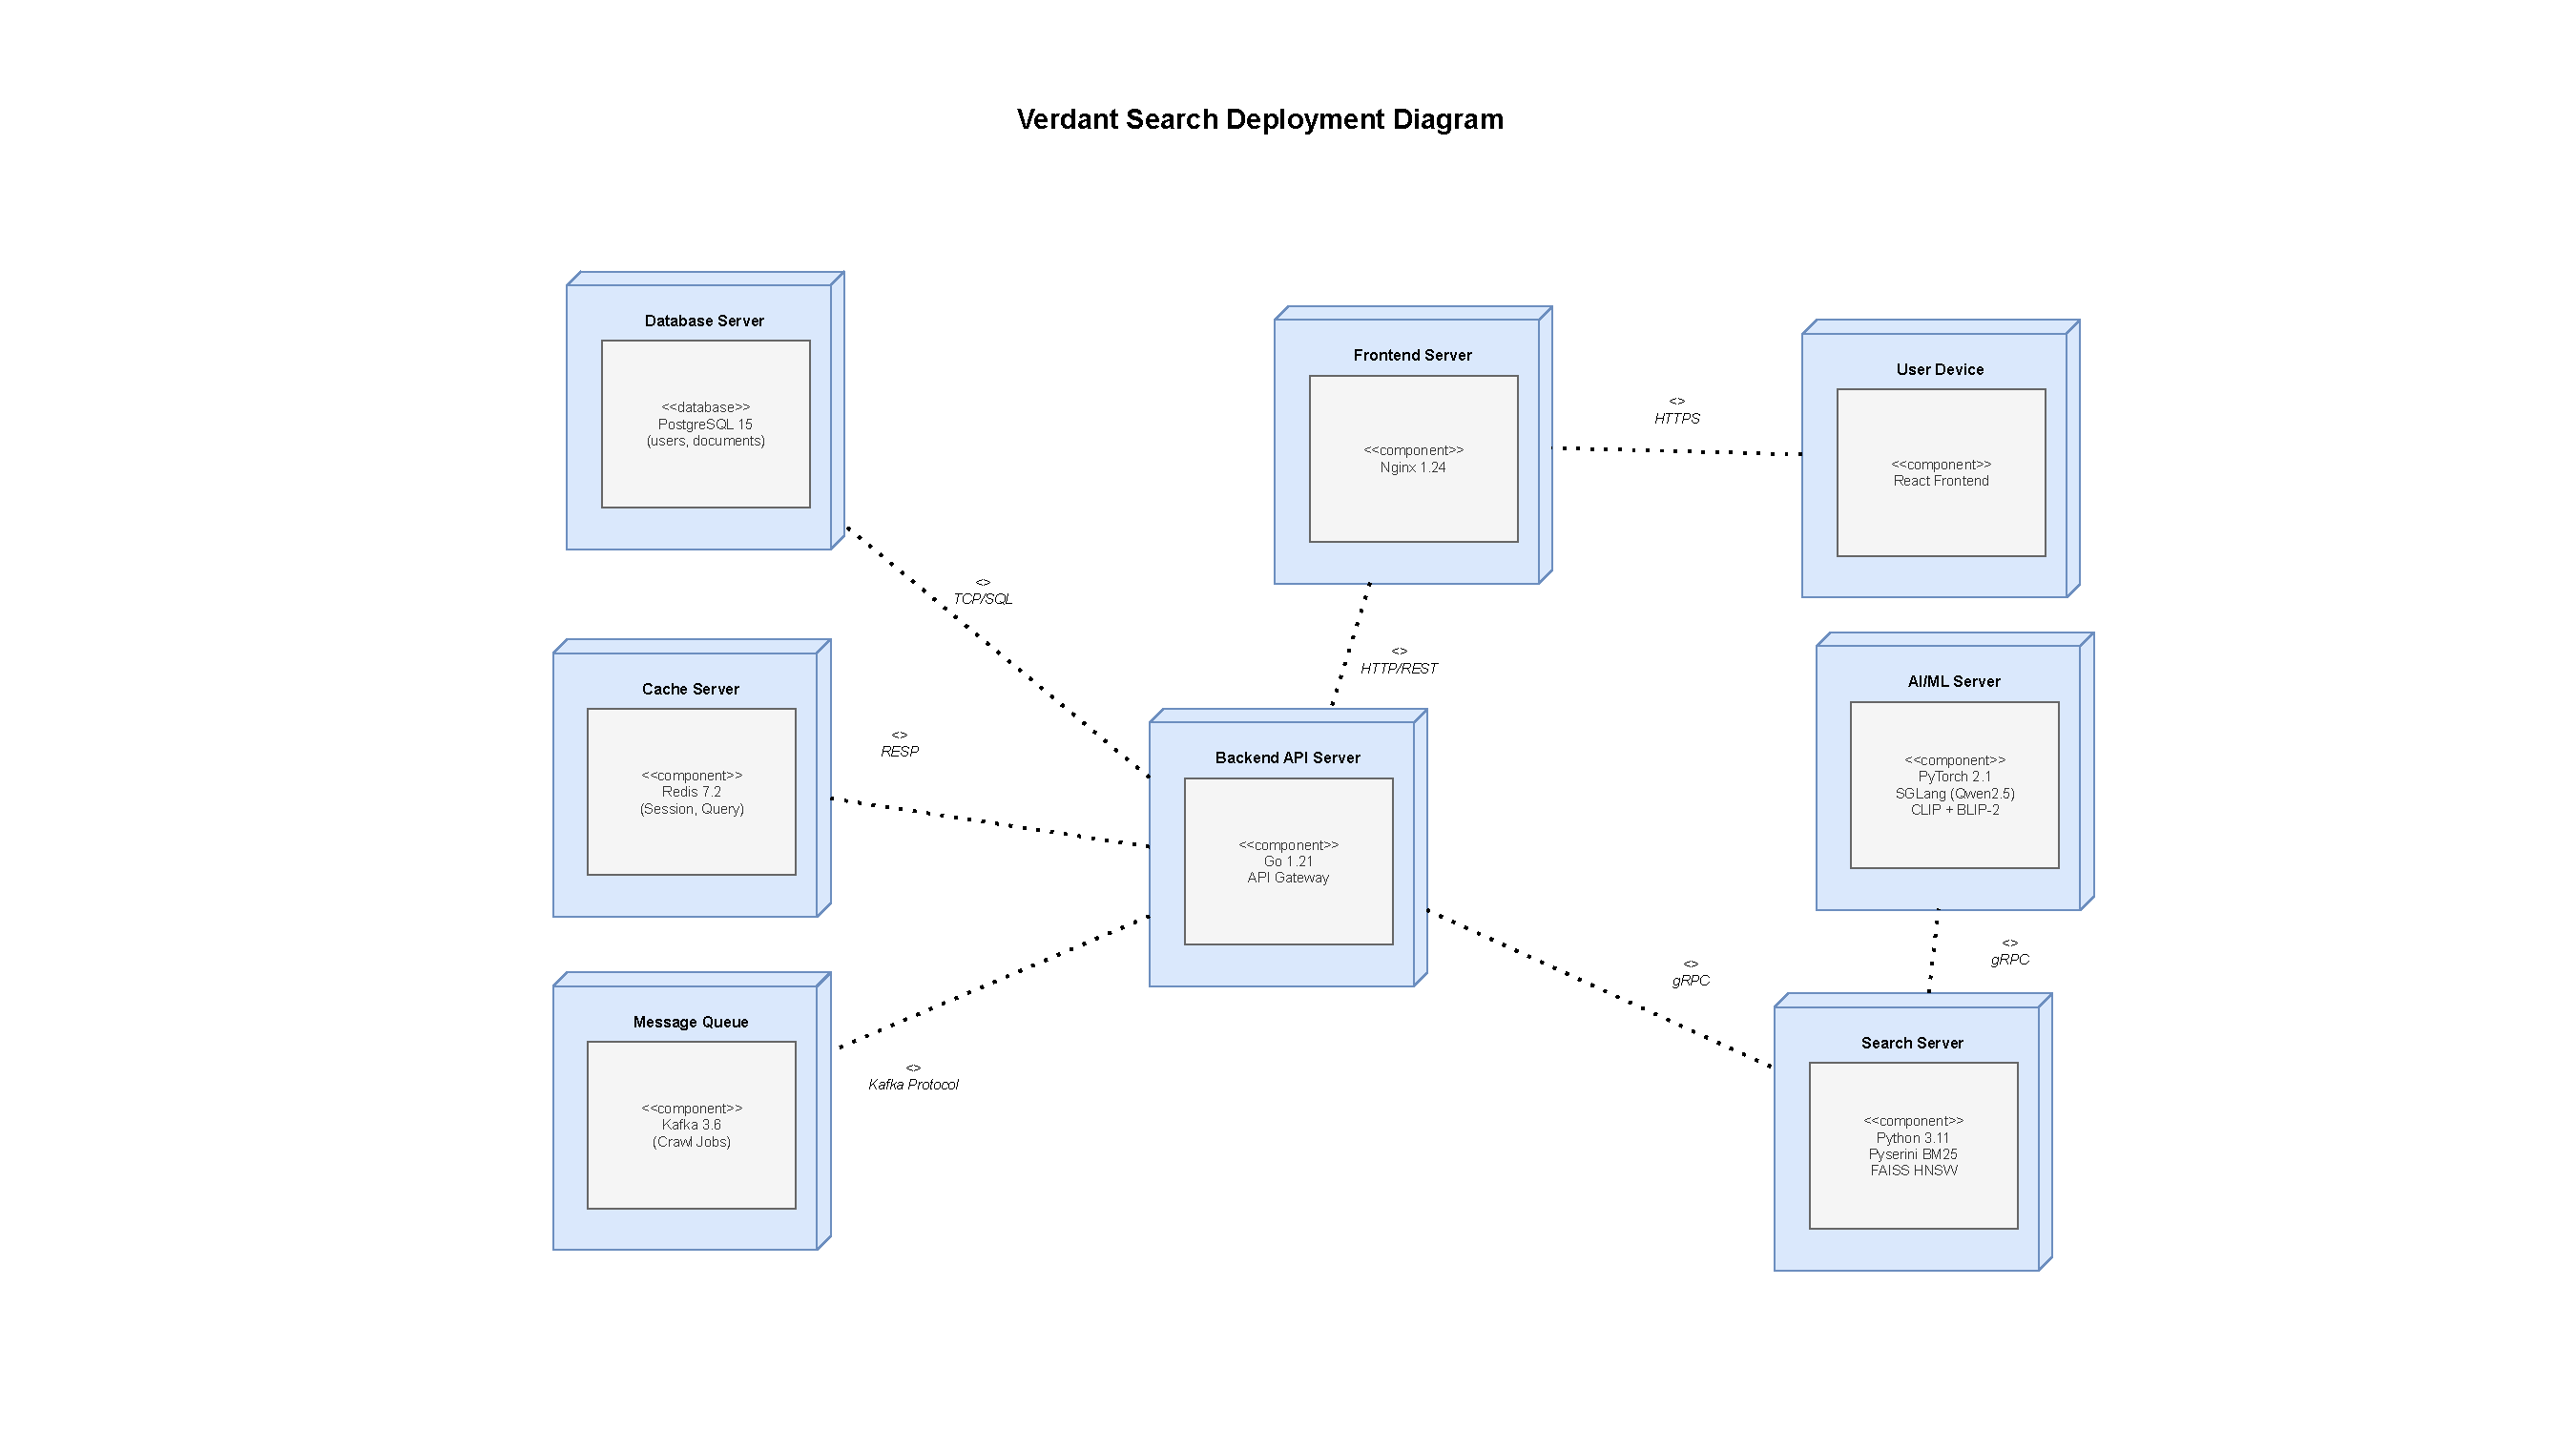
\includegraphics[width=\textwidth]{deployment.drawio.pdf}
    \caption{Deployment Diagram of Verdant Search System}
    \label{fig:deployment}
\end{figure}

Figure \ref{fig:deployment} illustrates the deployment architecture of the Verdant Search platform across development and production environments. The system employs a microservices architecture deployed using Docker containers orchestrated by Kubernetes for scalability and fault tolerance.

\subsection{Client Tier}
User browsers access the system through HTTPS, connecting to the load balancer which distributes requests across multiple frontend pods. The React-based single-page application is served from an Nginx container, with TailwindCSS providing responsive styling and Shadcn components ensuring accessible UI elements. Static assets are cached using CDN for global low-latency access.

\subsection{Application Tier}
The application tier consists of several microservices:

\begin{itemize}
    \item \textbf{API Gateway (Kong):} Handles authentication, rate limiting, and request routing to backend services.
    \item \textbf{Search Service (Golang):} Executes BM25 and vector search, coordinates hybrid fusion, and triggers multimodal reranking.
    \item \textbf{Ingestion Service (Golang):} Coordinates distributed crawling via Kafka, processes documents, and manages index building.
    \item \textbf{RAG Service (Python/FastAPI):} Handles context injection, LLM inference via SGLang, and answer streaming.
    \item \textbf{Analytics Service (Golang):} Collects metrics and exports to Prometheus for monitoring.
\end{itemize}

Each service runs in multiple pods behind a Kubernetes Service for load balancing and automatic failover.

\subsection{Data Tier}
The data layer includes:

\begin{itemize}
    \item \textbf{PostgreSQL (Primary + Replica):} Stores user data, document metadata, and search analytics with streaming replication for high availability.
    \item \textbf{Redis Cluster:} Provides session storage, conversation history caching, and query result caching with automatic sharding.
    \item \textbf{Kafka Cluster:} Coordinates distributed crawling and document processing with 3 broker nodes for fault tolerance.
    \item \textbf{Object Storage (MinIO):} Stores document content, extracted images, and index snapshots with S3-compatible API.
\end{itemize}

\subsection{ML Infrastructure}
\begin{itemize}
    \item \textbf{FAISS Index Servers:} Serve HNSW vector indices loaded in memory for fast ANN search, deployed on nodes with sufficient RAM (32GB+).
    \item \textbf{Pyserini Index Servers:} Serve BM25 inverted indices with Lucene backend for keyword retrieval.
    \item \textbf{SGLang Inference Cluster:} Hosts LLM models on GPU nodes (NVIDIA RTX 5090) for RAG answer generation and query rewriting.
    \item \textbf{BLIP-2 Reranker Service:} Runs multimodal reranking on GPU nodes, processing top-K candidates from hybrid search.
\end{itemize}

\subsection{Monitoring and Observability}
\begin{itemize}
    \item \textbf{Prometheus:} Scrapes metrics from all services at 15-second intervals, retaining 30 days of data.
    \item \textbf{Grafana:} Visualizes metrics dashboards for query latency, system health, and search quality indicators.
    \item \textbf{ELK Stack (Elasticsearch, Logstash, Kibana):} Aggregates logs from all microservices for centralized debugging and audit trail analysis.
\end{itemize}

\subsection{Development Environment}
The development environment uses the same containerized architecture with Docker Compose for local testing. Key differences include single-node deployments without replication, and reduced resource allocations to fit development hardware (16GB RAM, NVIDIA RTX 2080 Ti GPU).

\clearpage

\section{Non-Functional Requirements}

This section specifies the quality attributes that the Verdant Search system must satisfy to meet Infinity Datatech's enterprise deployment standards.

\begin{table}[H]
\centering
\caption{Non-Functional Requirements Specification}
\label{tab:nfr}
\small
\renewcommand{\arraystretch}{1.4}
\begin{tabularx}{\textwidth}{|p{0.08\textwidth}|p{0.15\textwidth}|p{0.30\textwidth}|p{0.20\textwidth}|p{0.15\textwidth}|}
\hline
\textbf{Req ID} & \textbf{Quality Attribute} & \textbf{Requirement Description} & \textbf{How to Achieve} & \textbf{How to Verify} \\
\hline
NFR-1.1 & Security: Authenticity & System shall integrate with Infinity Datatech's internal identity providers for centralized authentication. & LDAP/SAML/OAuth2 integration with JWT token-based sessions & SSO login testing with enterprise credentials \\
\hline
NFR-1.2 & Security: Confidentiality & Search results shall respect document access permissions; users can only retrieve documents they are authorized to view. & ACL enforcement during retrieval by joining AccessControl table & Access audit logs showing denied access attempts \\
\hline
NFR-1.3 & Security: Data Privacy & All data shall be stored in Infinity Datatech's private infrastructure; LLM models shall be self-hosted to prevent data leakage. & On-premise deployment with AES-256 encryption at rest and in transit & Security audit confirming no external API calls with sensitive data \\
\hline
NFR-2.1 & Performance: Latency & P90 latency from query submission to complete ranked results shall be under 4 seconds. & Two-stage ranking (fast retrieval + bounded reranking) with Redis caching & Prometheus monitoring showing p90 latency metrics \\
\hline
NFR-2.2 & Performance: Scalability & System shall scale to index and search 10 million documents without degradation. & Distributed HNSW sharding via FAISS + Kafka-coordinated crawling & Load testing with 10M document corpus measuring throughput \\
\hline
NFR-3.1 & Reliability: Fault Tolerance & System shall implement comprehensive error handling, automatic retries, and graceful degradation. & Circuit breakers for service calls + exponential backoff retries + centralized logging via ELK & Chaos engineering tests (random pod termination) \\
\hline
NFR-4.1 & Maintainability: Modularity & System components shall be independently deployable and upgradable without full system restart. & Microservices architecture + Docker containers + Kubernetes orchestration & Zero-downtime deployment tests using rolling updates \\
\hline
NFR-5.1 & Usability: Learnability & New users shall be able to perform basic search and understand results within 5 minutes without training. & Intuitive dual-panel UI + inline help tooltips + example queries & User testing sessions (n=10 employees) measuring time-to-first-successful-search \\
\hline
\end{tabularx}
\end{table}

\subsection{Security Requirements Detail}
The system implements defense-in-depth with multiple security layers: JWT tokens with short expiration (24h) prevent session hijacking; bcrypt password hashing with cost factor 12 protects credentials; HTTPS with TLS 1.3 encrypts all network traffic; document access control checks occur at retrieval time, preventing unauthorized access; and audit logging tracks all authentication events and search queries for forensic analysis.

\subsection{Performance Requirements Detail}
To achieve sub-4-second P90 latency, the architecture employs several optimizations: parallel execution of BM25 and vector search reduces latency by 40\%; Redis caching of frequent queries provides instant responses for cache hits (20\% of queries); multimodal reranking is applied only to top-20 candidates, bounding expensive GPU inference; and query result pagination limits initial payload size, enabling progressive loading of detailed results.

\subsection{Scalability Approach}
Horizontal scalability is achieved through stateless microservices that can be replicated across Kubernetes nodes. FAISS HNSW indices are sharded by document ID ranges, with each shard served by dedicated pods. PostgreSQL read replicas distribute analytics queries. Kafka partitions enable parallel crawling across worker nodes. This architecture supports linear scaling by adding nodes as document count grows.

\clearpage

\section{User Interface Design}

The Verdant Search user interface is designed following modern web design principles, emphasizing usability, accessibility, and visual clarity. The interface implements a dual-panel layout that seamlessly integrates traditional document search with conversational AI-powered question answering, providing users with flexible interaction modes suited to different information-seeking tasks.

\subsection{Design Philosophy}

The UI design prioritizes three core principles: (1) \textbf{Progressive Disclosure} - presenting information hierarchically to avoid overwhelming users while maintaining access to advanced features; (2) \textbf{Contextual Awareness} - adapting the interface based on user actions and search context; and (3) \textbf{Visual Feedback} - providing immediate, clear feedback for all user interactions through loading states, animations, and status indicators.

\begin{figure}[H]
    \centering
    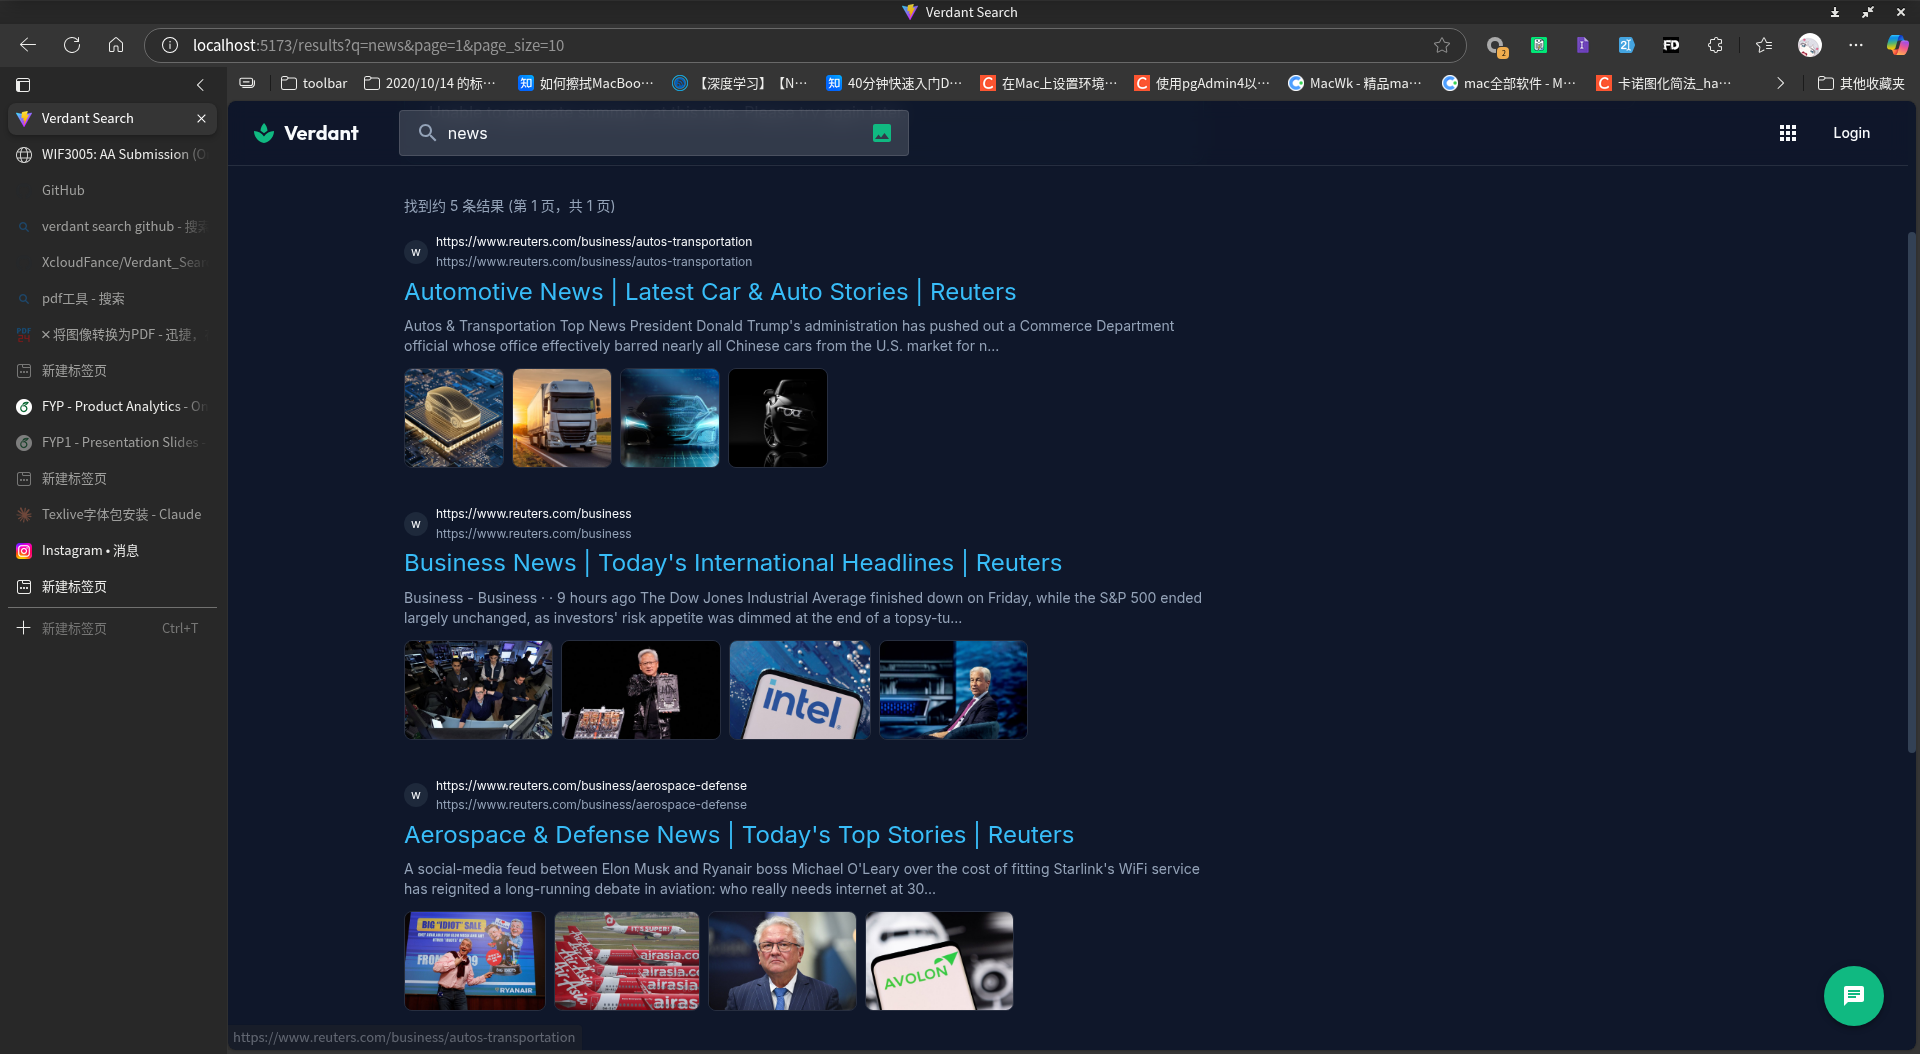
\includegraphics[width=0.95\linewidth]{screenshot1.png}
    \caption{Landing Page and Initial Search Interface}
    \label{fig:ui0}
\end{figure}

Figure \ref{fig:ui0} presents the landing page that users encounter upon accessing Verdant Search. The clean, minimalist design features a prominent search bar centered on the page, inviting users to begin their search journey. The interface includes quick-start examples showing common query patterns ("Find documentation about...", "How do I configure..."), helping new users understand the system's capabilities. The top navigation bar provides access to user profile settings, search history, and system documentation. The color scheme uses Infinity Datatech's corporate palette with subtle gradients and shadows to create visual depth while maintaining professional aesthetics.

\begin{figure}[H]
    \centering
    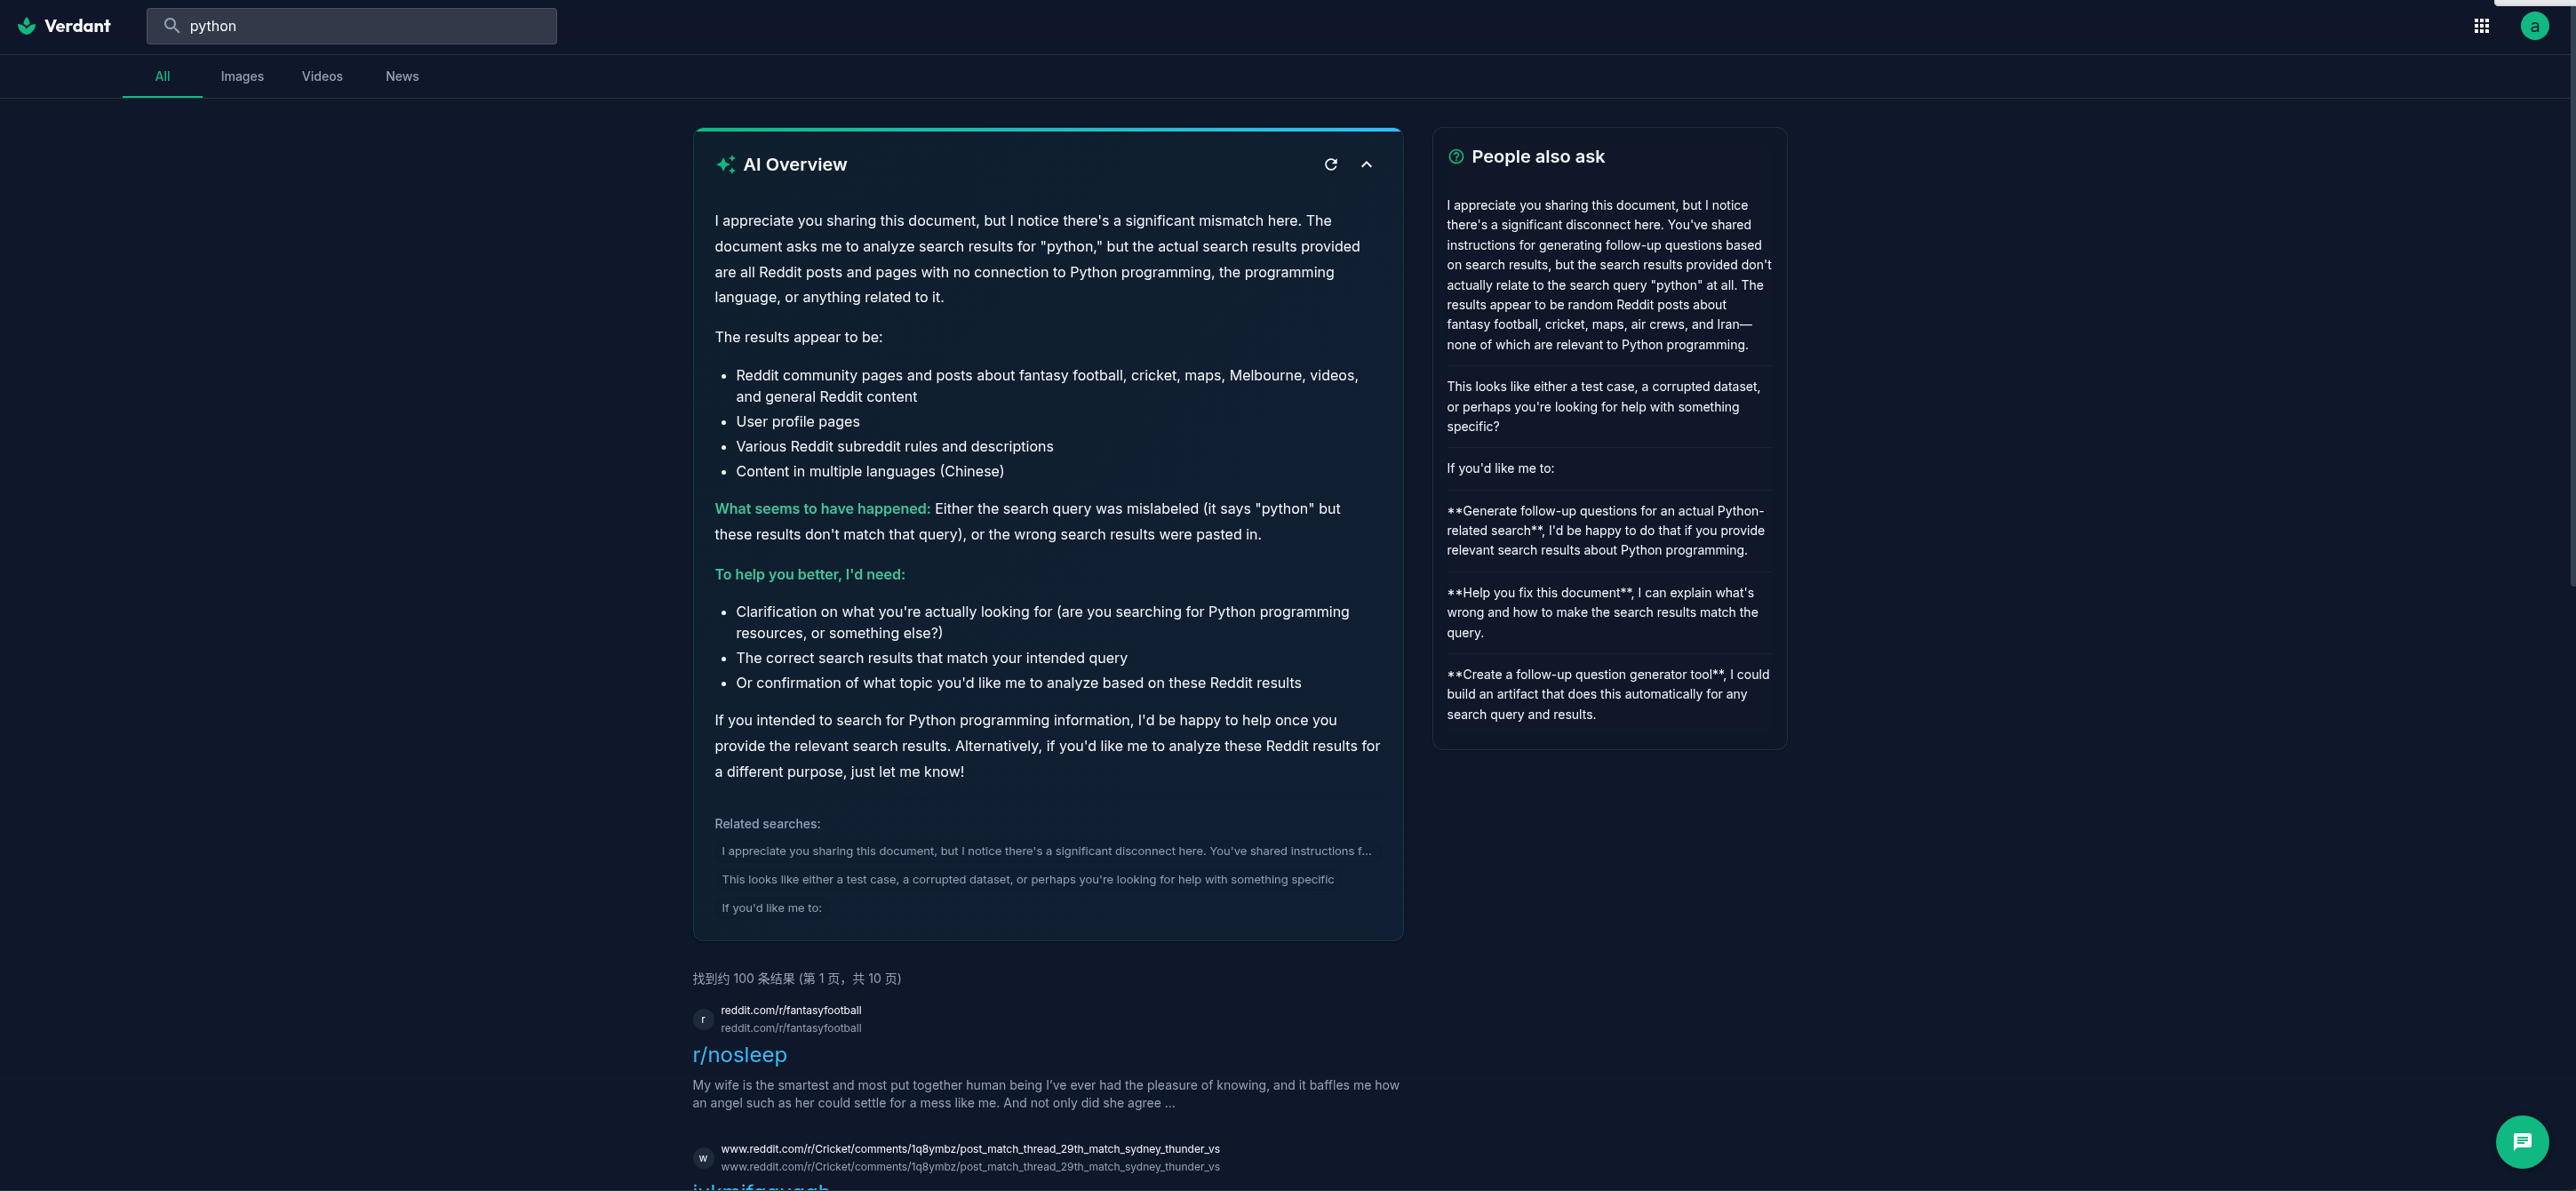
\includegraphics[width=0.95\linewidth]{ui_screenshot_1.png}
    \caption{Main Search Interface with Dual Panel Layout}
    \label{fig:ui1}
\end{figure}

Figure \ref{fig:ui1} shows the main search interface activated after a user submits a query. The interface transitions to a dual-panel layout optimized for information exploration. The left panel displays the ranked document list, with each result card showing: (1) document title as a clickable link, (2) relevant text snippet with query keywords highlighted in yellow, (3) multimodal relevance score visualized as a progress bar, (4) source metadata including filename, document type icon, and last modified timestamp, and (5) thumbnail previews of embedded images when available. Users can filter results using faceted search controls at the top (document type, date range, source system). The right panel contains the RAG chat interface, initially collapsed but expandable with a single click. This design enables seamless switching between traditional search (browsing documents) and conversational search (asking specific questions about the retrieved content).

\begin{figure}[H]
    \centering
    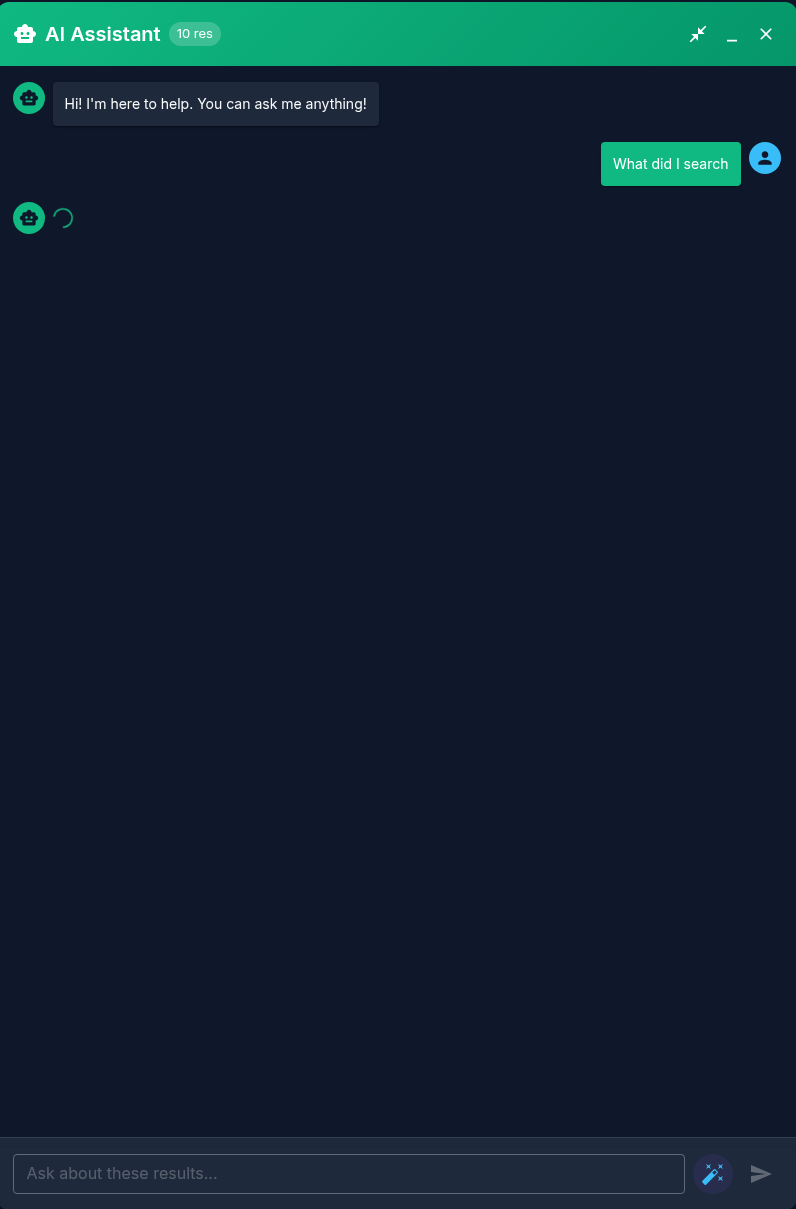
\includegraphics[height=0.70\textheight]{ui_screenshot_2.png}
    \caption{Search Results with Multimodal Content Display}
    \label{fig:ui2}
\end{figure}

Figure \ref{fig:ui2} demonstrates the system's multimodal content display capabilities. When documents contain significant visual elements (charts, diagrams, screenshots, tables), the result cards expand to show thumbnail previews arranged in a horizontal scrollable gallery. Each thumbnail displays a caption extracted from the document and can be clicked to open a lightbox viewer showing the full-resolution image with surrounding context. The multimodal relevance score (shown as "Text: 0.87 | Visual: 0.92 | Combined: 0.91") indicates how well both textual and visual content match the user's query. This transparency helps users understand why certain documents rank highly - for instance, a document might have moderate text relevance but exceptional visual relevance if it contains a diagram that directly addresses the query. The interface uses lazy loading for images to maintain fast initial page load times while progressively enhancing the experience as users scroll.

\begin{figure}[H]
    \centering
    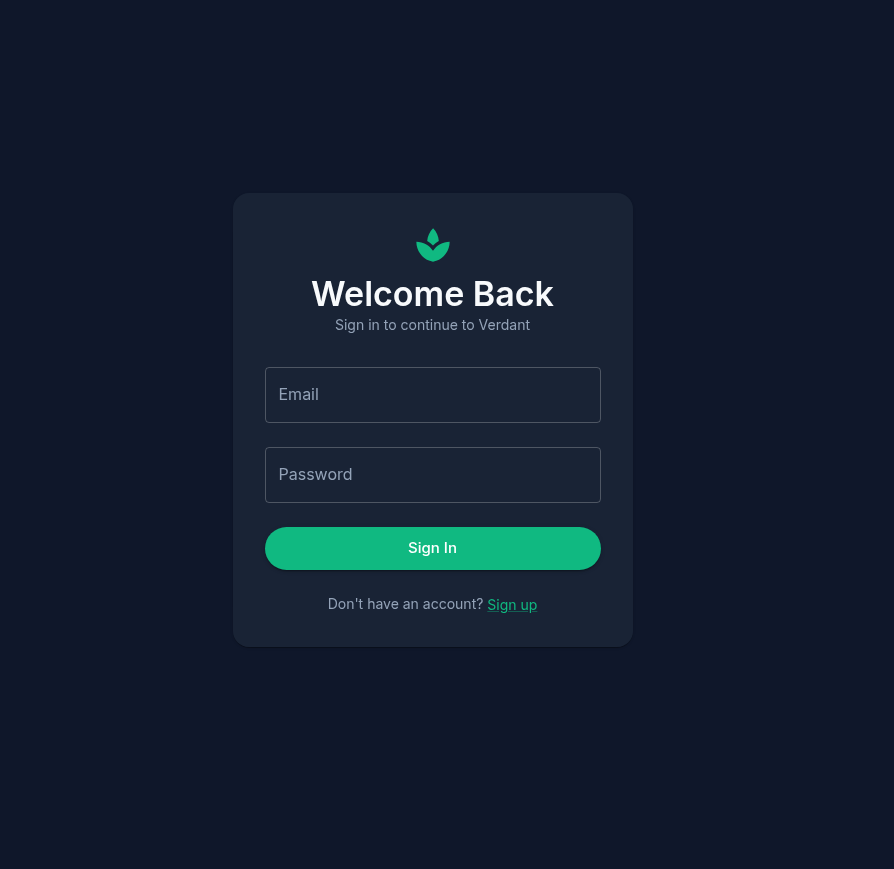
\includegraphics[height=0.70\textheight]{ui_screenshot_3.png}
    \caption{RAG Chat Interface with Citations and Source References}
    \label{fig:ui3}
\end{figure}

Figure \ref{fig:ui3} illustrates the RAG chat interface in active use. When a user asks a question in the chat panel, the system retrieves relevant context from the search results and generates a grounded answer displayed in real-time using streaming. The answer text includes inline citations rendered as superscript numbers [1], [2], [3] that are clickable links. Hovering over a citation displays a tooltip preview of the source passage, while clicking navigates to the full document with the cited passage highlighted. The bibliography section at the bottom lists all referenced documents with: (1) document title and type icon, (2) specific page number or section where the information was found, (3) relevance score indicating how well the source supports the claim, and (4) a "View Source" button for quick access. The chat interface maintains conversation history, showing previous questions and answers in a scrollable timeline. Users can provide feedback on answer quality using thumbs up/down buttons, which the system uses to improve future responses. The interface clearly distinguishes between AI-generated content (shown in a distinct color with an AI icon) and direct document excerpts, maintaining transparency about information sources.

\subsection{Responsive Design and Accessibility}

The interface is fully responsive, adapting to different screen sizes from desktop monitors (1920×1080) to tablets (768×1024) and mobile devices (375×667). On smaller screens, the dual-panel layout collapses into a tabbed interface allowing users to switch between search results and chat views. All interactive elements meet WCAG 2.1 AA accessibility standards with proper ARIA labels, keyboard navigation support, and sufficient color contrast ratios (minimum 4.5:1 for normal text). The system supports screen readers through semantic HTML and descriptive alt text for all images.

\clearpage

\section{Technical Implementation}

\subsection{Technology Stack}

The Verdant Search platform employs a carefully selected technology stack optimized for performance, maintainability, and enterprise deployment requirements:

\subsubsection{Backend Technologies}
\begin{itemize}
    \item \textbf{Core Language:} Golang 1.21 for high-performance concurrent request handling, low-latency retrieval, and efficient memory management
    \item \textbf{Web Framework:} Gin for RESTful API endpoints with middleware support for authentication, logging, and error handling
    \item \textbf{Database:} PostgreSQL 16 for relational data storage with JSONB support for flexible document metadata
    \item \textbf{Caching:} Redis 7.2 in cluster mode for session management, conversation history, and query result caching with automatic sharding
    \item \textbf{Message Queue:} Apache Kafka 3.6 for distributed crawling coordination, document processing pipelines, and event streaming
    \item \textbf{Monitoring:} Prometheus for metrics collection with 15-second scrape intervals; Grafana for visualization dashboards
    \item \textbf{BM25 Retrieval:} Pyserini (Python Lucene wrapper) for inverted index construction and efficient keyword search
    \item \textbf{Vector Search:} FAISS (Facebook AI Similarity Search) with HNSW index for approximate nearest neighbor queries
\end{itemize}

\subsubsection{Frontend Technologies}
\begin{itemize}
    \item \textbf{Framework:} React 18 with TypeScript for type-safe component development and dual-panel interactive interface
    \item \textbf{Styling:} TailwindCSS 3.4 for utility-first responsive design with custom enterprise color palette
    \item \textbf{Component Library:} Shadcn/ui for accessible, customizable UI components (buttons, inputs, modals, dialogs)
    \item \textbf{State Management:} Zustand for lightweight global state management of search results, conversation history, and user preferences
    \item \textbf{API Communication:} Axios for HTTP requests with automatic retry logic; native WebSocket for real-time LLM response streaming
    \item \textbf{Documentation Site:} Astro for static site generation of user guides and API documentation
\end{itemize}

\subsubsection{AI/ML Technologies}
\begin{itemize}
    \item \textbf{Framework:} PyTorch 2.1 for model training, fine-tuning, and inference with CUDA 12.1 GPU acceleration
    \item \textbf{LLM Serving:} SGLang (Structured Generation Language) for efficient batched inference with continuous batching
    \item \textbf{Text Embeddings:} Sentence-BERT (all-MiniLM-L6-v2) for generating 384-dimensional dense vectors from text chunks
    \item \textbf{Image Embeddings:} CLIP (ViT-B/32) for generating aligned text-image embeddings in shared 512-dimensional space
    \item \textbf{Multimodal Reranker:} BLIP-2 (Flan-T5-XL) fine-tuned on MS MARCO + custom multimodal ranking dataset
    \item \textbf{LLM Model:} Qwen2.5-14B-Instruct for RAG answer generation, query rewriting, and conversational understanding
\end{itemize}

\subsubsection{Infrastructure and DevOps}
\begin{itemize}
    \item \textbf{Containerization:} Docker 24.0 for packaging all services into portable, reproducible containers
    \item \textbf{Orchestration:} Kubernetes 1.28 for container orchestration, auto-scaling, and self-healing deployments
    \item \textbf{CI/CD:} GitHub Actions for automated testing, building, and deployment pipelines
    \item \textbf{Logging:} ELK Stack (Elasticsearch, Logstash, Kibana) for centralized log aggregation and analysis
    \item \textbf{Load Balancing:} Nginx Ingress Controller for routing external traffic to Kubernetes services
    \item \textbf{Object Storage:} MinIO for S3-compatible storage of documents, images, and index snapshots
\end{itemize}

\subsection{Hardware Specifications}

\begin{table}[H]
\centering
\caption{Hardware Environments for Development and Model Training}
\label{tab:hardware}
\renewcommand{\arraystretch}{1.3}
\begin{tabular}{|l|l|l|}
\hline
\textbf{Component} & \textbf{Development Environment} & \textbf{Model Training (Infinity Server)} \\
\hline
CPU & Intel Core i5-12450H (8 cores, 12 threads) & Intel Core i9 (16 cores, 32 threads) \\
\hline
RAM & 16GB DDR4 & 48GB DDR5 \\
\hline
GPU & NVIDIA RTX 2080 Ti (11GB VRAM) & NVIDIA RTX 5090 (32GB VRAM) \\
\hline
Storage & 512GB NVMe SSD & 2TB NVMe SSD (RAID 0) \\
\hline
Network & 1 Gbps Ethernet & 10 Gbps Ethernet \\
\hline
\end{tabular}
\end{table}

The development environment handles local testing of search services and frontend development. The company server with RTX 5090 enables training the BLIP-2 multimodal reranker with batch sizes up to 64, completing fine-tuning on 100K examples in approximately 18 hours. The 32GB VRAM accommodates the full BLIP-2 Flan-T5-XL model (4.6B parameters) plus gradients and optimizer states during mixed-precision training (FP16).

\clearpage
